\chapter{Methods}\label{ch:Methods}
% In this chapter, we first introduce necessary mathematical and algorithmic foundations to provide an in-depth view of our algorithm's core components and explain their relevance in the new approach. 
In this chapter, we propose a novel approach/concept to create a universal clustering result w.r.t.\ combining a local density-based clustering approach with a global correlation clustering one. For this purpose, we first introduce the necessary mathematical and algorithmic foundations to provide an in-depth view of our algorithm's core components, specifically elaborate on them further by giving a detailed explanation to their functionalities and explain their relevance to our concept. With this knowledge/expertise, we offer a, to the best of our knowledge, the first approach by combining mentioned components and visualizing the single steps to present a more thorough view, with regards to the underlying clustering structure, of the procedure. \todor{v2 in comments}
\todor{bin mir nich sicher ob first tho}
% In this chapter, we propose a novel approach/concept to create a universal clustering result by combining a local correlation clustering approach with a global one. For this purpose, we first introduce necessary mathematical and algorithmic foundations to provide an in-depth view of our algorithm's core components. We then specifically elaborate on them further by giving a detailed explanation to its functionality and explaining their relevance to our concept and offer a first approach by combining mentioned components and visualizing the single steps to present a more intuitive view of the procedure. 


% In this chapter 
% Clustering in Arbitrary Subspaces based on the Hough transform (CASH) is cool; however, its complexity is $\mathcal{O}(n^2)$.
% We try to do it better by using a density-based approach to prune away irrelevant points and noise.

\section{Mathematical and Algorithmic Foundations}
\label{sec:Foundations}
Our Algorithm builds on top of two algorithms which both were built on two other well-known algorithms: \gls{optics}, which is closely related to \gls{dbscan}, and \gls{cash}, which is inherently based on the Hough transform.

\subsection{DBSCAN - In Depth}
\label{ssec:DBSCANindepth}
\begin{figure}
    \centering
    \begin{minipage}{.47\textwidth}
      \centering
      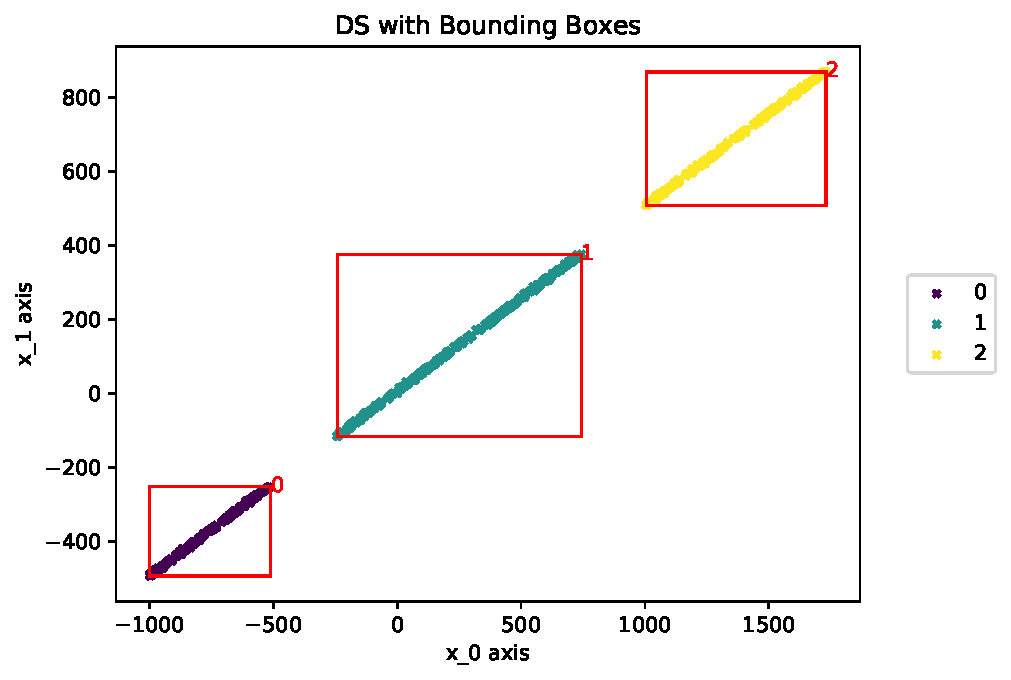
\includegraphics[width=.8\textwidth]{figures/DSwithDBSCANBoundingBoxes.pdf}
      \captionsetup{width=0.8\linewidth}
      \captionof{figure}{Density-based clustering without Noise}
      \label{fig:cleandbscan}
    \end{minipage}%
    \begin{minipage}{.53 \textwidth}
      \centering
      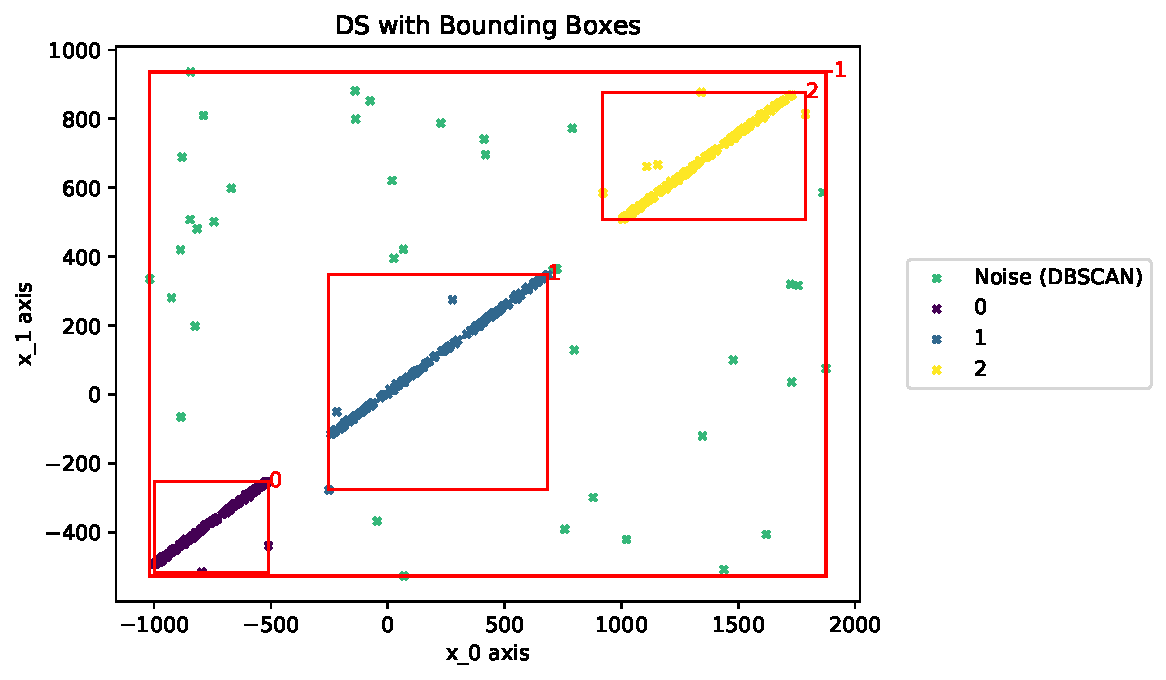
\includegraphics[width=.8\textwidth]{figures/DBSCANwithNoise.pdf}
      \captionsetup{width=0.8\linewidth}
      \captionof{figure}{Density-based clustering with Noise}
      \label{fig:noisydbscan}
    \end{minipage}
\end{figure}
To begin with, we decided to utilize \gls{dbscan} to retrieve the dense intervals of the original data set. 
As mentioned before the algorithm \gls{dbscan} is categorized into the density-based approach of clustering. 
This means that it considers a set of points connected through low proximity in a restricted area/space into similar clusters and thus can, in contrast to traditional partitioning based approaches, create clusters of arbitrary shape (cf. \autoref{fig:kmeansdbscan}). 
Hence these clusters can retain more accurate information about the correlation of the data. Additionally, it also directly eliminates noise and can, therefore, lower the computational cost of the future steps. 
Its basic principle is as follows:
A group of points is considered a dense cluster when for each point of the cluster, there are sufficient other points in its neighbourhood~\cite{DBSCANEKSX96}.

To understand how this algorithm works, we first have to introduce some terminology.
Given a data set $DS$ of data objects $o$ with a dimensionality of $N$, a distance measure $dist(p_1,p_2)$ and two new parameters, the Epsilon distance $\epsilon$ and the minimum number of points to be a cluster $MinPts$, \citeauthor{DBSCANEKSX96} defines:

\subsubsection*{$\epsilon$-Neighbourhood}
% \begin{defn}
The $\epsilon$-Neighbourhood $N_{\epsilon}(p)$ of a point $p$ is defined by the set of points $q$ which have a smaller distance $dist(p,q)$ than the threshold $\epsilon$. Formally: 
% \[N_{\epsilon}(p)=\{q \in DS \mid dist(p,q) \leq \epsilon\}\]
\begin{align}
    N_{\epsilon}(p)=\{q \in DS \mid dist(p,q) \leq \epsilon\}
\end{align}

This measure alone, however, is not enough to fully cluster dense groups, since it would only register points inside the cluster (core points) and omit those at the border of the clusters (border points) since they have fewer points in their neighbourhood. To include those border points too, \citeauthor{DBSCANEKSX96} introduce three more properties/relationships between points.
% \end{defn}

\subsubsection*{(Direct) Density-Reachability}
The direct density-reachability of a point $p$ from another point $q$ is fulfilled if:
% \begin{enumerate}
%     \item $p \in N_{\epsilon}(q)$
%     \item \label{eq:minptsreq}\(|N_{\epsilon}(q)|\geq MinPts\)
% \end{enumerate}
% \begin{flalign}
%     &p \in N_{\epsilon}(q)\label{eq:pinN}&\\\vspace{2mm}
%     &|N_{\epsilon}(q)|\geq MinPts\label{eq:minptsreq}&
% \end{flalign}
\begin{align}
    p \in N_{\epsilon}(q)\label{eq:pinN}\\
    |N_{\epsilon}(q)|\geq MinPts\label{eq:minptsreq}
\end{align}
where \autoref{eq:minptsreq} represents the condition for point \(q\) to be a core point. If a point \(p\) is in the $\epsilon$-Neighbourhood of a core point $q$, but itself is not a core point, then point $p$ is labelled as a border point. 

\todor{original sounds way better}
A target point $p$ is density-reachable from origin point $q$, if there exists a sequence of connecting points $p, c_1, \dotsc, c_n, q$ in between $p$ and $q$ which are directly density-reachable to its predecessor, e.g. $c_1$ is directly density-reachable from point $q$, $c_2$ is directly density-reachable from point $c_1$, \dots\todor{format} until $p$ is directly density-reachable from point $c_n$. This relation is obviously transitive, but only symmetric if both points of the relation are core points. In case of a border point as the origin, there are not enough points in its neighbourhood and therefore it does not have any density-reachable neighbour as a target to start with.

\todor{own fig}
\begin{figure}
    \centering
    \begin{subfigure}[t]{.5\textwidth}
      \centering  
      \captionsetup{width=.9\linewidth}
      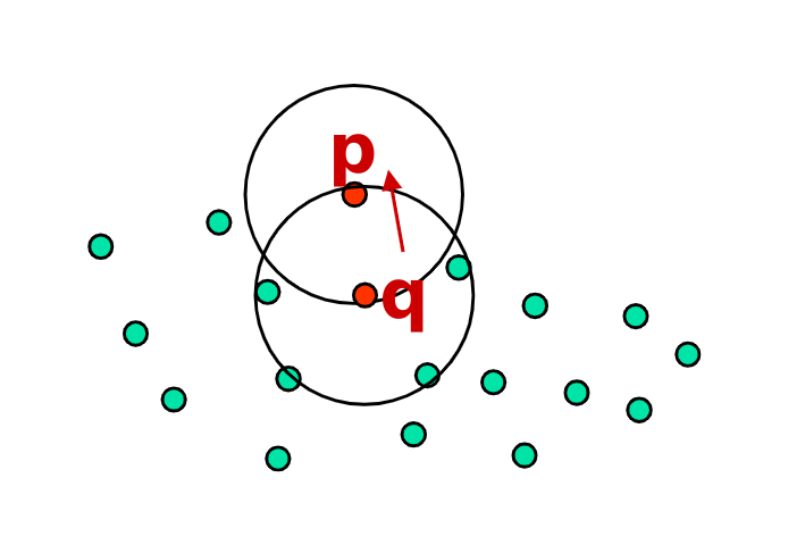
\includegraphics[width=.8\textwidth]{figures/directlydensityreachable.png}
      \caption{Border point p is directly density-reachable from core point q.}
      \label{fig:directdensityreachable}
    \end{subfigure}%
    \begin{subfigure}[t]{.5\textwidth}
      \centering
      \captionsetup{width=.9\linewidth}
      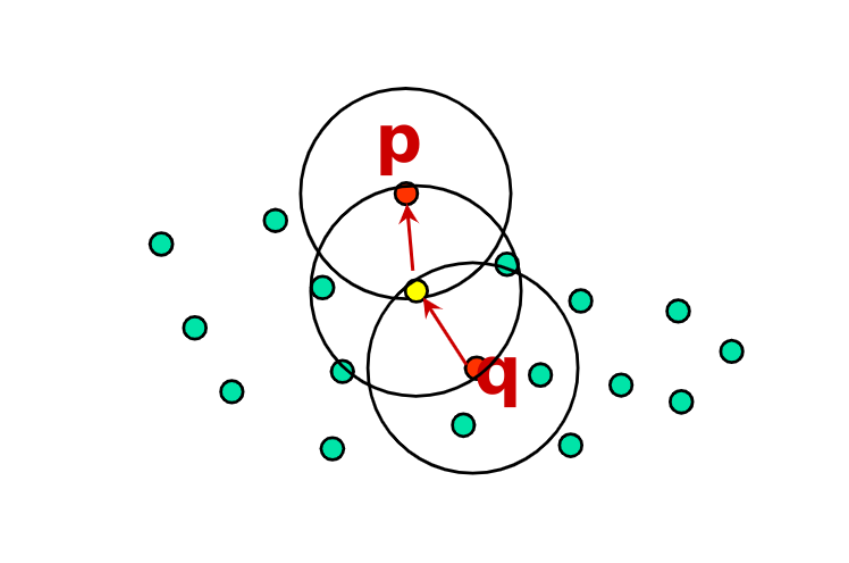
\includegraphics[width=.8\textwidth]{figures/density-reachable.png}
      \caption{p is not directly density-reachable, but density-reachable from q.}
      \label{fig:densityreachable}
    \end{subfigure}
    \caption{Illustration of reachabilities wrt. $\epsilon$ and $MinPts = 3$, src: KDD-VL.}
\end{figure}

\subsubsection*{Density-Connectedness}
The last relation between points is the density-connectedness. Two points $p$ and $q$ are density-connected, if there exists a point $c$, where both points $p$ and $q$ are density-reachable from point $c$. In contrast to the (direct) density-reachability, this relation is symmetric and even reflexive if both points $p$ and $q$ are density-reachable from each other. \todo{generate wider figure saving some space}
\begin{figure}
    \centering
    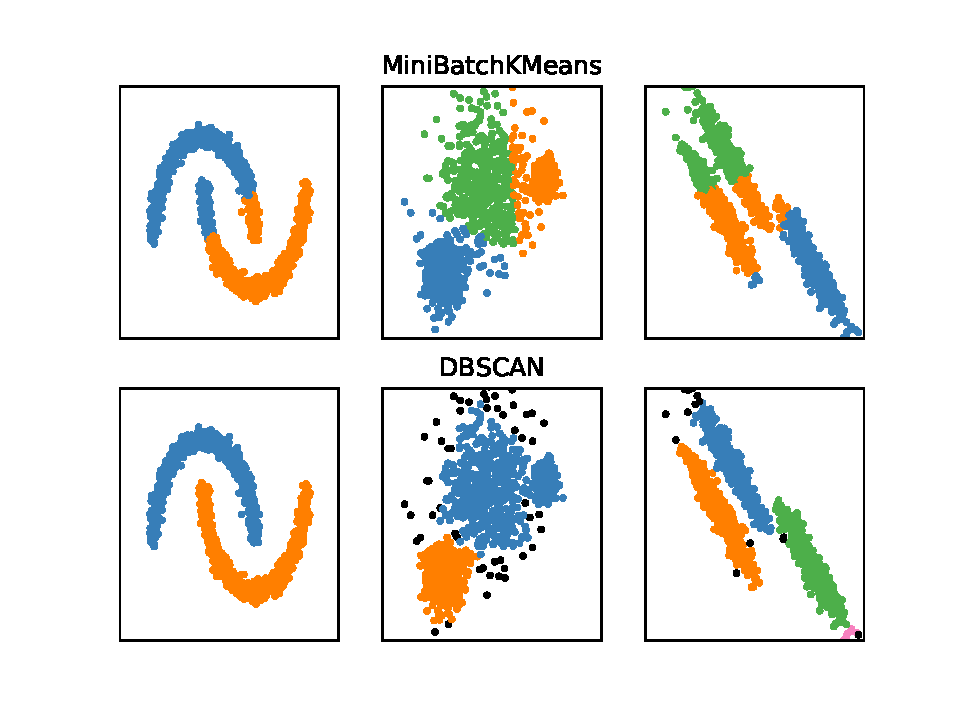
\includegraphics[width=0.7\textwidth]{figures/KMeansVSDBSCAN.pdf}
    \caption{Density-based clustering compared to partitioning clustering.}
    \label{fig:kmeansdbscan}
\end{figure}

\vspace{5mm}

Given the previously defined relations, we can now define the notion of clusters and noise in \gls{dbscan}:

\subsubsection*{Density-based Clusters}
A dense cluster is the union of a set of density-connected core points $CP$ and the set of border points $BP$ which are density-reachable from $CP$.
Formally \citeauthor{DBSCANEKSX96} defines a \gls{dbscan}-cluster as:

A dense cluster in data set $DS$ is a non-empty subset $C^{DB} \subseteq DS$ of points $p$ and $q$ if the following two conditions are fulfilled:
\todor{verbatim definition!}
% \begin{enumerate}
%     \item $\forall p, q$: if $p \in C$ and $q$ is density-reachable from $p$, then $q \in C$ (Maximality)
%     \item $\forall p, q \in C$: $p$ is density-connected to $q$ (Connectivity)
% \end{enumerate}
\begin{align}
    &\forall p, q: \text{if } p \in C^{DB} \text{ and } q \text{ is density-reachable from } p \text{, then } q \in C^{DB} \\
    &\forall p, q \in C^{DB}: p \text{ is density-connected to }q
\end{align}

This definition of clustering therefore defines any cluster with \textit{at least} a density defined by the Epsilon-distance $\epsilon$ and the number of minimum points $MinPts$.

\subsubsection*{Density-based Noise}
Every point not belonging to any of the existing clusters $C^{DB}_1, \dotsc, C^{DB}_k$ in data set $DS$ are now considered noise: 
\begin{align}
    noise^{DB} = \{p \in  DS | \forall i : p \notin C^{DB}_i\}
\end{align}
\todob{transition?}

\subsubsection*{The DBSCAN-Algorithm}
One way to calculate the clusters using \gls{dbscan} is as follows:

First, select the first point $p$ of data set $DS$ and check its $\epsilon$-neighbourhood. Save every neighbour into a seed list/queue $L$ for further evaluation and check if the neighbourhood $N_{\epsilon}(p)$ has enough points to satisfy the $MinPts$-property. 
If it satisfies the property, then point $p$ is a core point and creates a new dense cluster. As long as the seed list is not empty every next point in the list is then classified as either part of the current cluster or noise.
However, if $N_{\epsilon}(p)$ does not satisfy the $MinPts$-property, then point $p$ is prematurely labelled as noise. This status will be changed, if another point $q$ has $p$ in its $\epsilon$-neighbourhood and itself is a core point, then it is relabelled as a border point of the current cluster.

Then the next point from the seed list $L$ is selected, and the same procedure is applied again.
If the seed list $L$ is empty, the current cluster is done, the next not previously observed point from $DS$ is evaluated, and the whole cycle repeats again until there is no point in the data set $DS$ left.

\vspace{5mm}
\begin{algorithm}[H]
% \algsetup{linenosize=\tiny}
% \scriptsize
\SetAlgoLined
% \DontPrintSemicolon
\KwData{data set $DS$; seed list $L$; current cluster $C^{DB}_i$; Noise $N^{DB}$; $MinPts$; $\epsilon$}
\KwResult{A set $R$ of clusters $C^{DB}_1,\dotsc,C^{DB}_n$ and noise $N^{DB}$}
 o := first Point of $DS\setminus \{R \cup N\}$\;
 L := [o]\;
 i := 0\;
 \While{$DS\setminus \{R \cup N\}$ is not empty}{
    \While{L is not empty}{
        currentPoint := L.pop(0)\;
        L.push($N_{\epsilon}(currentPoint)$)\;
        \eIf{$|N_{\epsilon}(currentPoint)| > MinPts$}{
            $C^{DB}_i$.add(currentPoint)\;
            $C^{DB}_i$.addAllNeighbors($N_{\epsilon}(currentPoint)$)\;
            N.removeAllNeighbors($N_{\epsilon}(currentPoint)$)\;
        }{
            N.add(currentPoint)
        }
    }
    R.add($C^{DB}_i$)\;
    o := first Point of $DS\setminus \{R \cup N\}$\;
    L := [o]\;
    i := i + 1\;
 }
 \caption{DBSCAN}
\end{algorithm}
\vspace{5mm}

This algorithm was the first approach to segmenting the original data space into subintervals of importance. However, there is a drawback with using \gls{dbscan} as the first segmentation. \gls{dbscan} relies on a global parameter setting which can only find clusters with approximately the same density or higher (c.f. \autoref{fig:DBSCANhierarchy}) and therefore would not be able to find the intrinsic clustering structure well if the underlying models of the global correlations created linear correlations with different densities. 
Note, however, that in increasing-dimensional spaces, the volume of the space increases exponentially fast, which causes the data space to become sparse. This induces that our data space might not be clusterable by a density-based approach in high-dimensional spaces. This phenomenon is also called the \textit{Curse of Dimensionality}~\cite{bellman2015adaptive}.

\begin{figure}
    \centering
    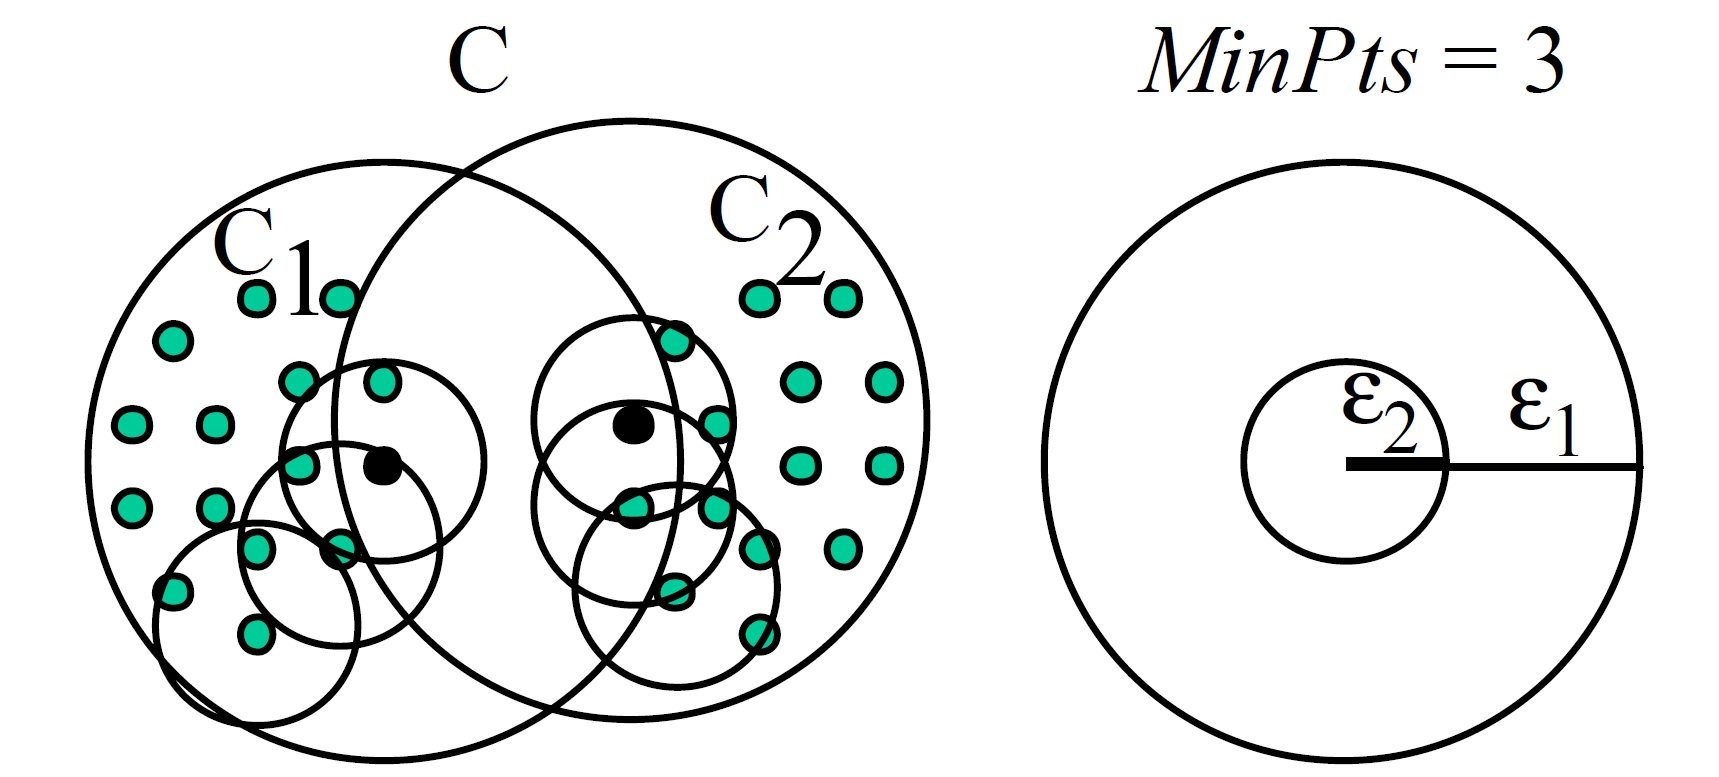
\includegraphics[width=.5\textwidth]{figures/DBSCANleastdensity.png}
    \caption{Hierarchical density: Different $\epsilon$-distances capture different clusters~\cite{opticsankerst1999optics}.}
    \label{fig:DBSCANhierarchy}
\end{figure}

\subsection{OPTICS - In Depth}\label{ssec:OPTICSindepth} \todob{check comment}%OPTICS ONLY wide range of epsranges, not different minpts, since reachability is dependent on minpts, it extends epsilon, if minpts is not satisfied
To tackle the detection of different densities, we replaced \gls{dbscan} with a more versatile algorithm/extension called \textit{\acrfull{optics}}. This algorithm has the capabilities to not only detect clusters of varying densities more accurately but also to keep open more possibilities for different further approaches for future work, e.g. a more extensive (bottom-up/hierarchical) approach by evaluating more density-settings at once based on different $\epsilon$-ranges.

Although \gls{optics} itself is not a clustering algorithm, it does create an ordering of the points in a database, which represents the density-based clustering structure of a wide range of $\epsilon$-parameter settings, with which it is possible to automatically create a more accurate clustering with different densities compared to \gls{dbscan}~\cite{opticsankerst1999optics}. To create such a consistent ordering \todo{cite style} \citeauthor{opticsankerst1999optics} defines the following two distances on top of the previously mentioned definitions of \autoref{ssec:DBSCANindepth}:
\vspace{5mm}

Given a point $p$ from the data set $DS$, an epsilon-distance $\epsilon$, the \todor{format} $\epsilon$-neighbourhood of $p$ $N_{\epsilon}(p)$, the minimum number of points to be a cluster $MinPts$ and the distance measure from $p$ to its $MinPts$-nearest neighbors $MinPts$-$dist(p)$. Then:
\todo{DBSCAN with one whole cluster instead of 2 separate}
\todor{Figure without bounding box}
\begin{figure}
    \centering
    \begin{minipage}{.54\textwidth}
      \centering
      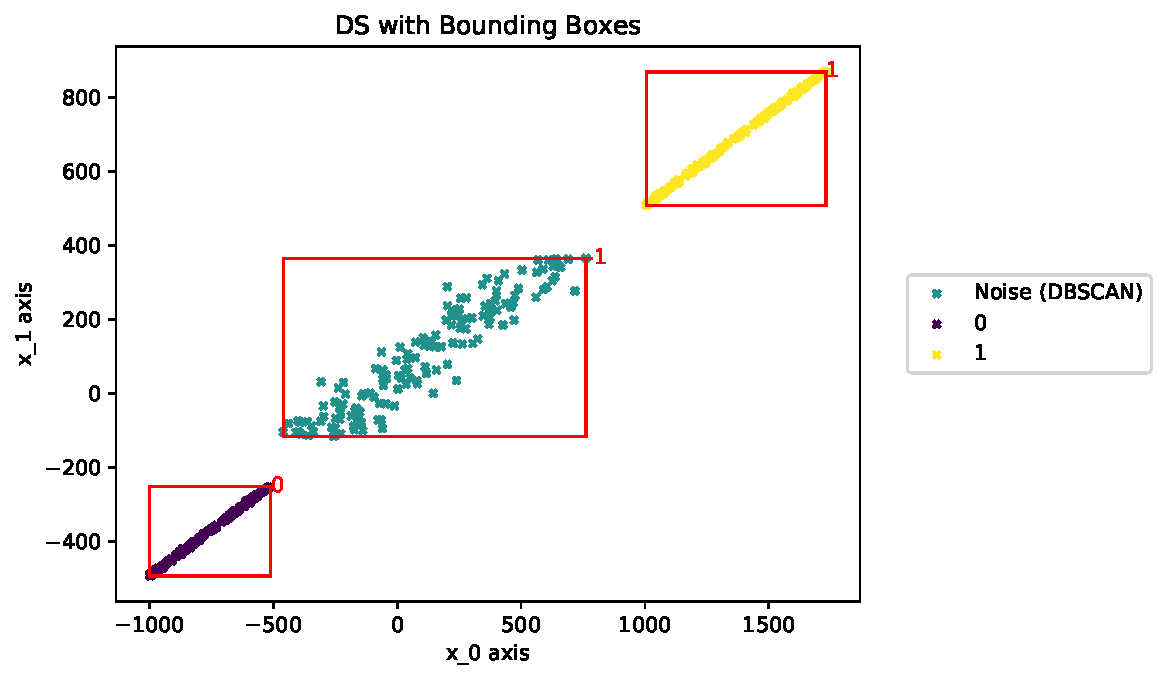
\includegraphics[width=.95\textwidth]{figures/DSwithDBSCANbadBoundingBoxes.pdf}
      \captionsetup{width=0.8\linewidth}
      \captionof{figure}{\acrshort{dbscan} detects sparser cluster as noise.}
      \label{fig:baddbscan}
    \end{minipage}%
    \begin{minipage}{.46\textwidth}
      \centering
      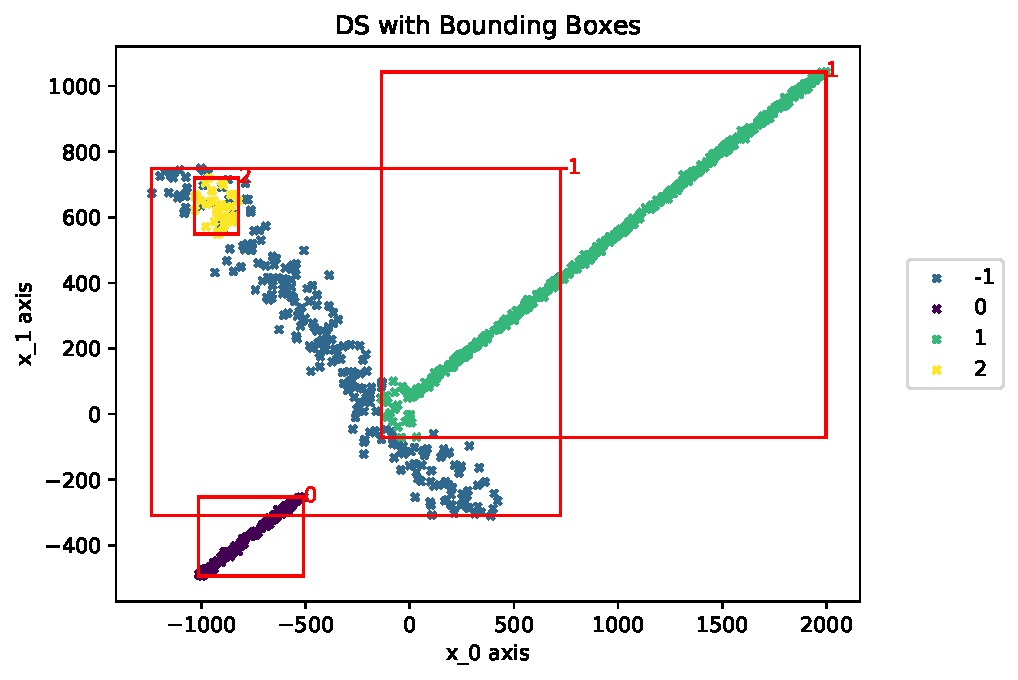
\includegraphics[width=.95\textwidth]{figures/DSwithOPTICSBoundingBoxes.pdf}
      \captionsetup{width=0.9\linewidth}
      \captionof{figure}{Separation of different dense clusters by using \acrshort{optics}.}
      \label{fig:goodoptics}
    \end{minipage}
\end{figure}

\subsubsection*{Core-Distance}
The core-distance of point $p$ describes the smallest distance $\epsilon_{core}$ with an upper bound of $\epsilon$ such that the number of points in $N_{\epsilon_{core}}(p)$ is greater than $MinPts$, i.e.\ $\epsilon_{core}$ is the smallest epsilon-distance possible for $p$ to be a core point w.r.t.\ to $\epsilon$ and $MinPts$. If $\epsilon_{core}$ exceeds $\epsilon$, then the core-distance of $p$ is \textit{undefined}. Formally the core-distance of p is defined as:
\begin{align}
    core\text{-}dist_{\epsilon,MinPts}(p)=
    \begin{cases}
        \text{undefined} &\text{if } |N_\epsilon(p)| < MinPts\\
        MinPts\text{-}dist(p) &\text{otherwise}
    \end{cases}
\end{align}

\subsubsection*{Reachability-Distance}
The reachability-distance of point $p$ w.r.t.\ another point $q$ is the smallest possible $\epsilon_{reach}$-distance with a lower bound of $core-dist(q)$ such that p is directly-density reachable from q. If $core-dist(q)$ is \textit{undefined}, then $q$ is not a possible core point and the $reach-dist(p,q)$ is also \textit{undefined}.
Formally the reachability-distance of $p$ w.r.t.\ $q$ is defined as:
\begin{align}
    reach\text{-}dist_{\epsilon,MinPts}(p,q)=
    \begin{cases}
        \text{undefined} &\text{if } |N_\epsilon(q)| < MinPts\\
        max(core\text{-}dist(q), dist(p,q)) &\text{otherwise}
    \end{cases}
\end{align}

\subsubsection*{The OPTICS-Algorithm} %This first processed point sound weird
The \gls{optics}-algorithm maintains two data structures to create the ordering, one seed list $L$, which contains (point, reach-dist)-tuples and is ordered by the reach-dist, and the cluster ordering list $O$. 
To create this ordering, \gls{optics} first initializes the ordering $O$ with the first point $o_{proc}$ of $DS$ and a reach-dist of $\infty$. A reachability-distance of $\infty$ from point $a$ w.r.t.\ point $b$ describes, that point $a$ is not contained in the $\epsilon$-neighbourhood of $b$ and therefore connected to the dense cluster. Since $o_{proc}$ is the first point of the ordering, it does not have a previous cluster to connect to and will never be in the reachability-distance of another point in the ordering. This first point in processing $o_{proc}$ now populates the ordered seed list $L$ with points $o_i$, belonging to the $\epsilon$-neighbourhood $N_\epsilon(o_{proc})$, and its reachability-distance w.r.t.\ $o_{proc}$, i.e.\ $reach$-$dist(o_i, o_{proc})$. The further iterations now depend on the state of the seed list $L$. Whenever $L$ is not empty, each next point $o_{proc}$ chosen for processing is taken from the ordered seed list and inserted into the cluster ordering list $O$ with its respective reachability-distance. If $L$ is empty, there is no candidate left to be density-connected and the next unprocessed point is chosen from $DS$ as a new $o_{proc}$ and inserted into $O$ with a reachability-distance of $\infty$ again. The point in process $o_{proc}$ is then used again to populate the seed list. This loop continues until there are no unprocessed points in $DS$ left.

\vspace{5mm}

\begin{algorithm}[H]
% \algsetup{linenosize=\tiny}
% \scriptsize
\SetAlgoLined
\KwData{data set $DS$; seed list $L$ ordered by reach-dist(); cluster order $O$; min \# of pts for a cluster $MinPts$; Eps-distance $\epsilon$}
\KwResult{Ordering $O$ representing the density-based clustering structure}
 L := $\emptyset$\;
 \While{$DS\setminus \{L \cup O\}$ is not empty}{
    \eIf{$L$ is empty}{
        o := next unprocessed Point of $DS\setminus \{L \cup O\}$\;
        $reach$-$dist$ := $\infty$\;
        $O$.append((o,$reach$-$dist$))\;
    }{
        (o, $saved\ reach$-$dist)$) := $L$.pop(0)\;
        $O$.append((o, $reach$-$dist(o)$))
    }
    \ForEach{$p \in N_\epsilon(o) \setminus \{$O$\}$}{
        $L$.update(($p$, $reach$-$dist(p, o)$))\;
    }
 }
 \caption{OPTICS}
\end{algorithm}
\vspace{5mm}
\todob{maybe chapter about reachability plots}

As an illustration \gls{optics} can visualize the hierarchy using a \textit{reachability plot} (c.f. \autoref{fig:reachabilityplot}).\\

All in all, \gls{optics} provides a more capable clustering tool for different densities, with an, in practice, only 1.6 higher runtime compared to its ancestor \gls{dbscan}. In theory, the runtime complexity of \gls{optics} is heavily dominated by the runtime of the neighbourhood query. Given a tree-based spatial index structure for the neighbourhood query, the runtime becomes $\mathcal{O}(|DS| \log |DS|)$, in the worst-case however the complexity raises to $\mathcal{O}(|DS|^2)$. Nonetheless, similar to \autoref{ssec:DBSCANindepth}, \gls{optics} also suffers from the \textit{Curse of Dimensionality}.

\begin{figure}
    \centering
    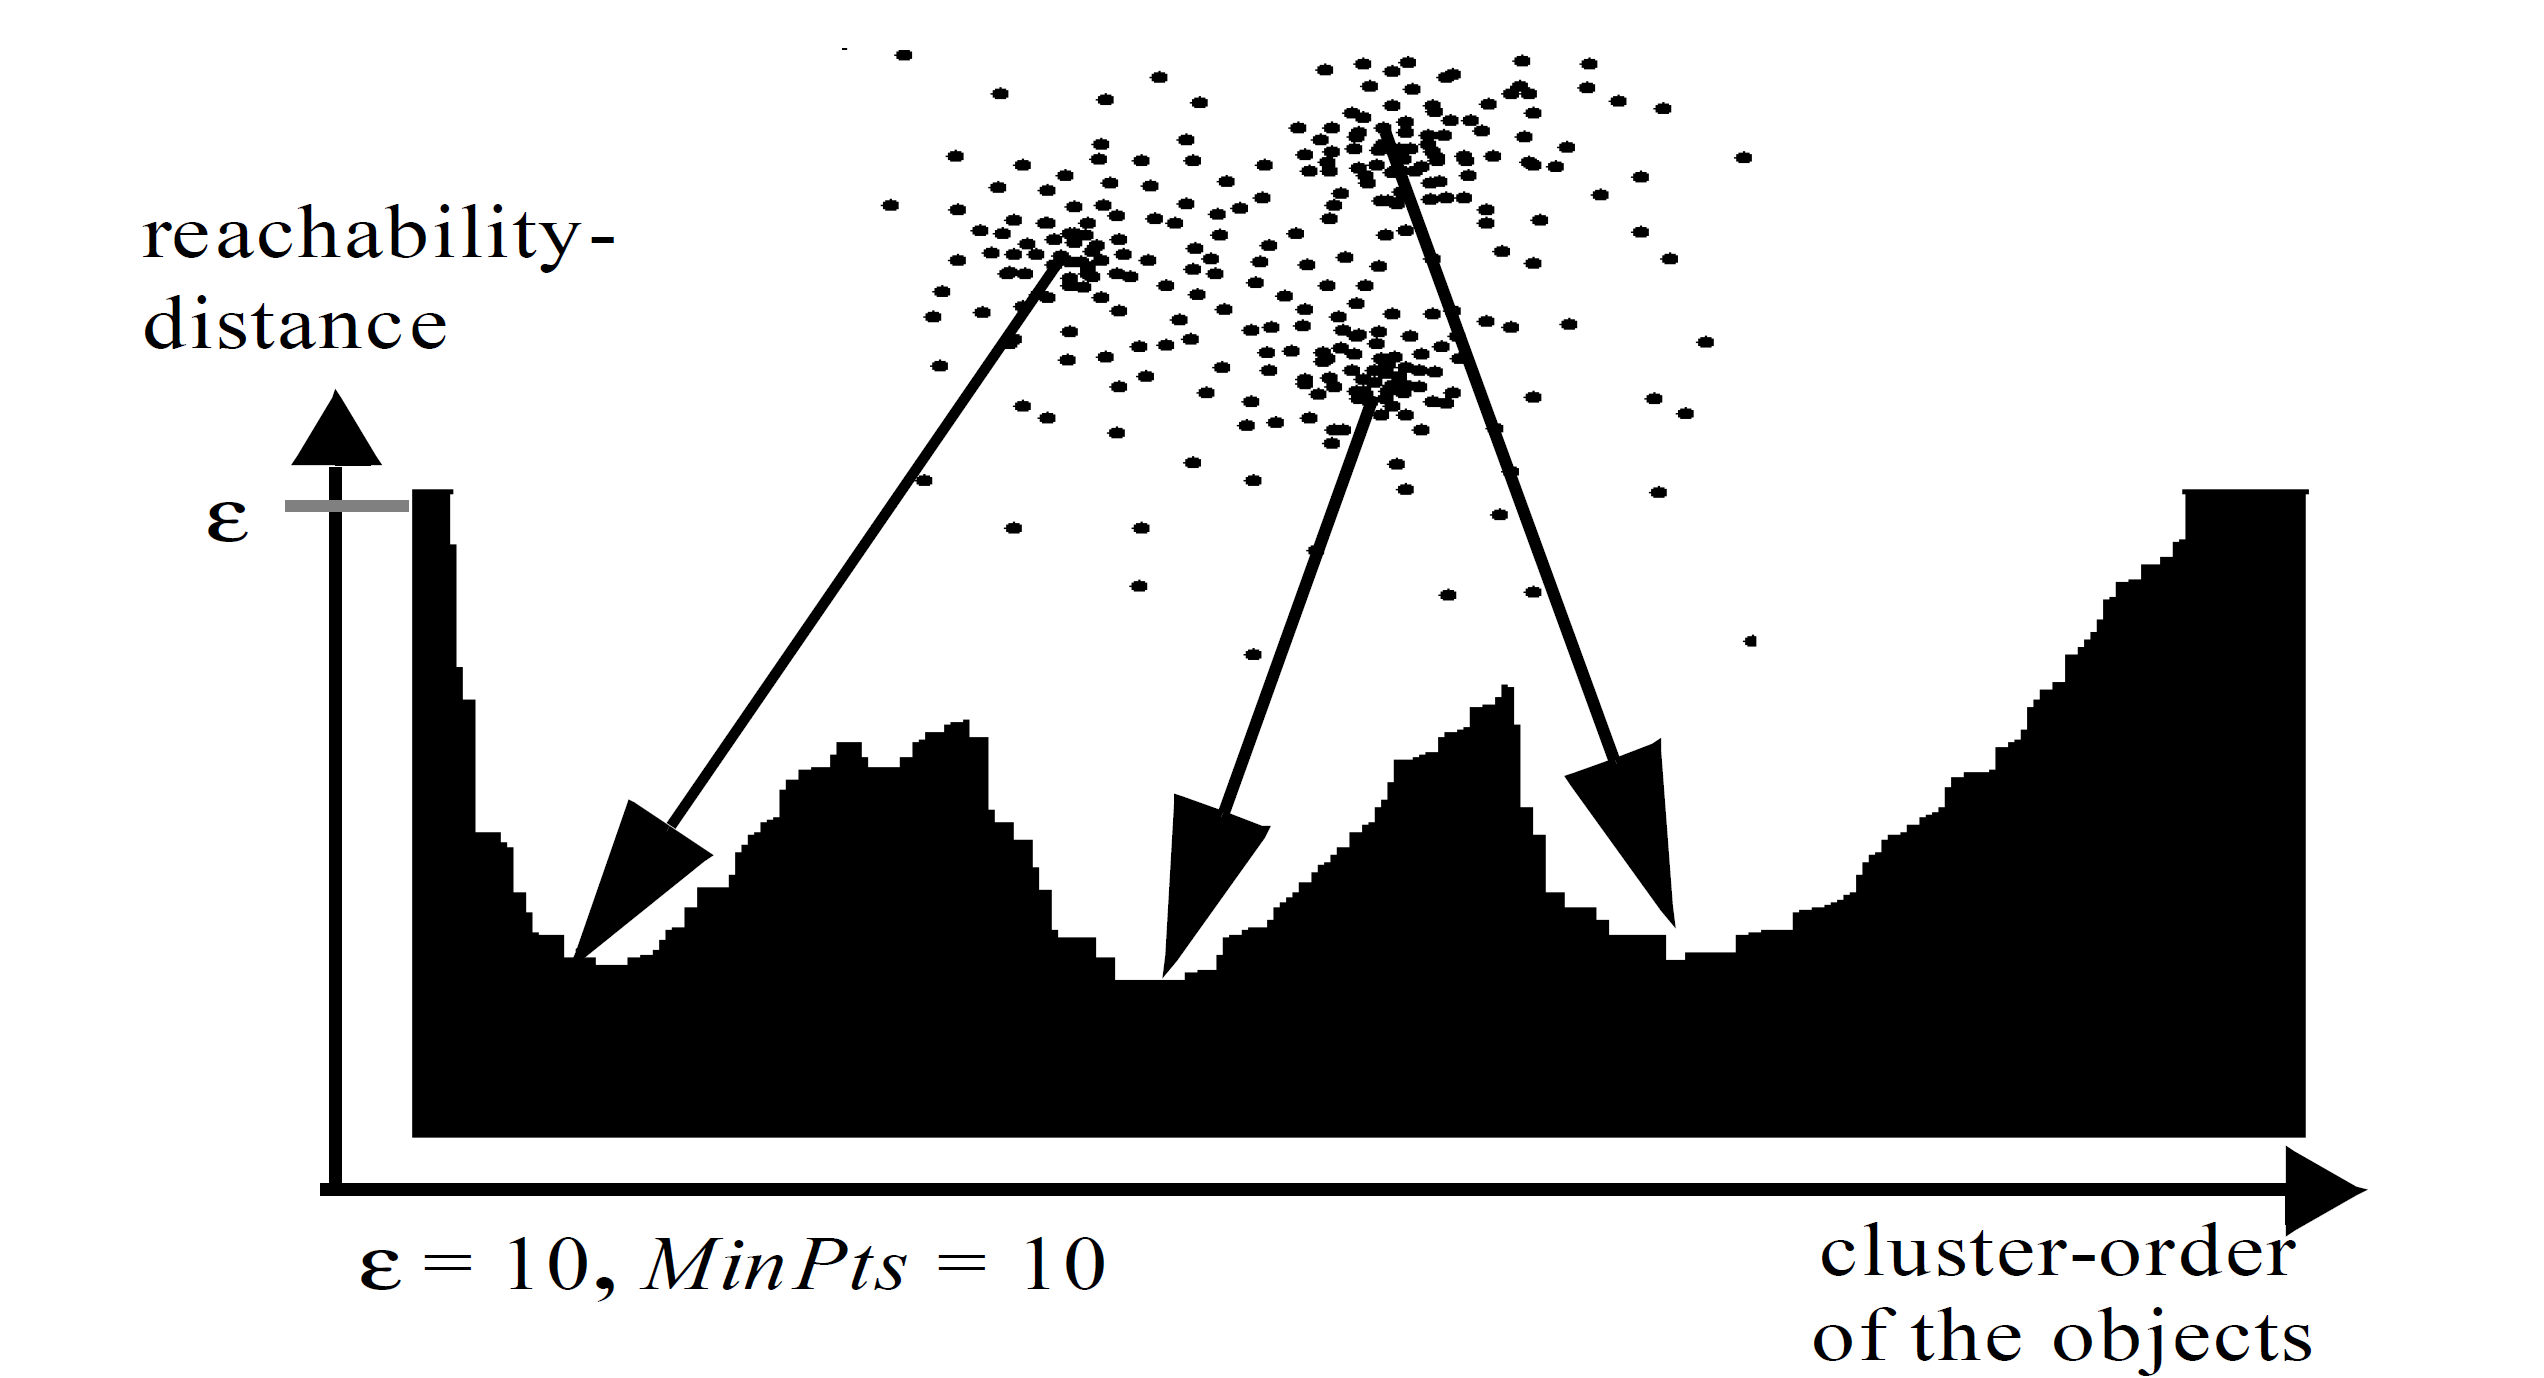
\includegraphics[width=0.7\textwidth]{figures/reachabilityplot.png}
    \caption{\acrshort{optics} ordering visualized as reachability plot. Valleys represent connected points with similar dense neighbourhoods~\cite{opticsankerst1999optics}.}
    \label{fig:reachabilityplot}
\end{figure}

\subsection{Hough Transformation - In Depth}\label{ssec:houghindepth}
The initial purpose of the Hough transform was a technique to detect colinear points~\cite{houghOriginal1962method} and has since then found various other applications in fields like image processing/analysis~\cite{rosenfeld1969picture,ballard1981generalizing}, computer vision~\cite{davies2004machine} and correlation clustering~\cite{CASHachtert2008robust}.
% \subsubsection{The basic idea}
The basic idea was the transformation of 2-dimensional points $p_i = (x_i,y_i)$ in data space $\mathcal{D} \subseteq \R^2$ with x and y axis to functions in the form of ${m_{p_i}(t_{p_i}) = \frac{y_i}{x_i} - \frac{t_{p_i}}{x_i}}$ in parameter space $\mathcal{P} \subseteq \R^2$, also known as Hough space, with t and m axis, where $m$ is the slope and $t$ is the y-intercept of a line passing through point $p_i$~\cite{illingworth1988survey}. It can be visualized by imagining that each point $p_i$ can be explained by an infinite number of concurrent lines $C$ defined by the functions 
\begin{align}
    {y_{p_i}(m,x) = m \cdot (x - x_i) + y_i}
\end{align}

If we only consider the value of $x=0$ we can still uniquely characterize each equation and instead of the y-value $y_{p_i}$ get the y-intersect $t$ w.r.t.\ slope $m$:
\begin{align}\label{eq:houghparamspace}
\begin{split}
y_{p_i}(m,0) 
&= m \cdot (0 - x_i) + y_i\\
&= -x_i \cdot m + y_i = t(m)
\end{split}\\
\label{eq:hougheq}
\Rightarrow m_{p_i}(t_{p_i}) &= \frac{y_i}{x_i} - \frac{t_{p_i}}{x_i}
\end{align}

A point $p_i = (x_i, y_i)$ in data space is then characterized by each possible $(m,t)$-setting of \autoref{eq:houghparamspace}. In parameter space these continuous $(m_{p_i},t_{p_i})$-settings are uniquely defined by the function in \autoref{eq:hougheq}. A point in data space therefore can be represented as a line in the $(m,t)$-parameter space (c.f.\ \autoref{fig:houghmxt}). \todob{graphing tool} %https://www.yworks.com/products/yed.

\begin{figure}
    \centering
    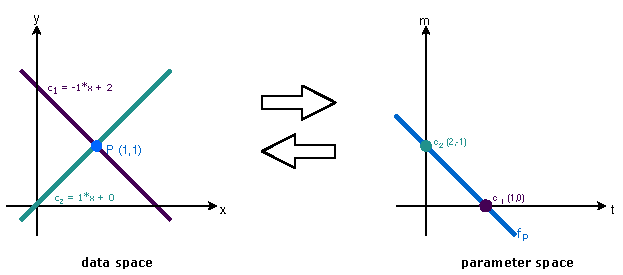
\includegraphics{figures/HoughMXT.pdf}
    \caption{Duality of the Hough transform: from (y,x)-space to (m,t) and back.}
    \label{fig:houghmxt}
\end{figure}

However using the slope-intercept form $y = m \cdot x + t$ comes with a drawback, it can not show lines parallel to the y-axis. As a solution, \citeauthor{duda1971use} propose the use of the \gls{hnf} for the concurrent lines instead. Their equations in data space change to the following form:
\begin{align}\label{eq:hnfangles}
    \begin{split}
        \delta_{p_i}(\theta_{p_i}) &= x_i \cos{\theta_{p_i}} + y_i \sin{\theta_{p_i}}\\
        &= f_{p_i}(\theta_{p_i})
    \end{split}
\end{align}
where $\delta$ denotes the shortest distance from the respective line to the origin and $\theta$ its respective angle. The parameter space therefore changes to a \mbox{$(\theta,\delta)$-parameter space} and points in data space are transformed to sinusoidal curves instead (c.f.~\autoref{fig:TODOHOUGH}). \todog{own fig}
Since the settings $(\theta,\delta)$ and $(\theta+k\pi,-2\delta)$ represent the same line, $\theta$ is restricted to the interval $[0,\pi)$. Given a point $p_i$ and all angles $\theta_{i,j}$, the distances $\delta_{i,j}$ can be calculated with \autoref{eq:hnfangles}. Hence the parameter space $\mathcal{P}$ can be bounded by $\mathcal{P} = [\delta_{min}, \delta_{max}]\times [0,\pi)$ where $\delta_{min}$ represents the global minimum and $\delta_{max}$ represents the global maximum of all functions $f$ w.r.t.\ all points. For easier illustration the angle $\theta$ can be transformed into a unit normal vector $\vec{n_0}$ (c.f.\ \autoref{eq:hnfunv}). \todo{hnf fig with $(\theta,\delta)$ and $(\vec{n},\delta)$}

\begin{align}
    \delta &= x_i \cos{\theta} + y_i \sin{\theta}\nonumber\\
    \text{substit}&\text{ute:}\ n_x = \cos{\theta},\ n_y = \sin{\theta} \nonumber\\
    \delta &= x_i n_x + y_i n_y\nonumber\\
    \label{eq:hnfunv}
    \delta &= \langle\vec{n_0},\vec{x}\rangle 
\end{align}

\begin{figure}
    \centering
    % \includegraphics{}
    \missingfigure{hnf visualizations in 2d}
    \caption{Caption}
    \label{fig:hnf_euclid}
\end{figure}

\begin{figure}
    \centering
    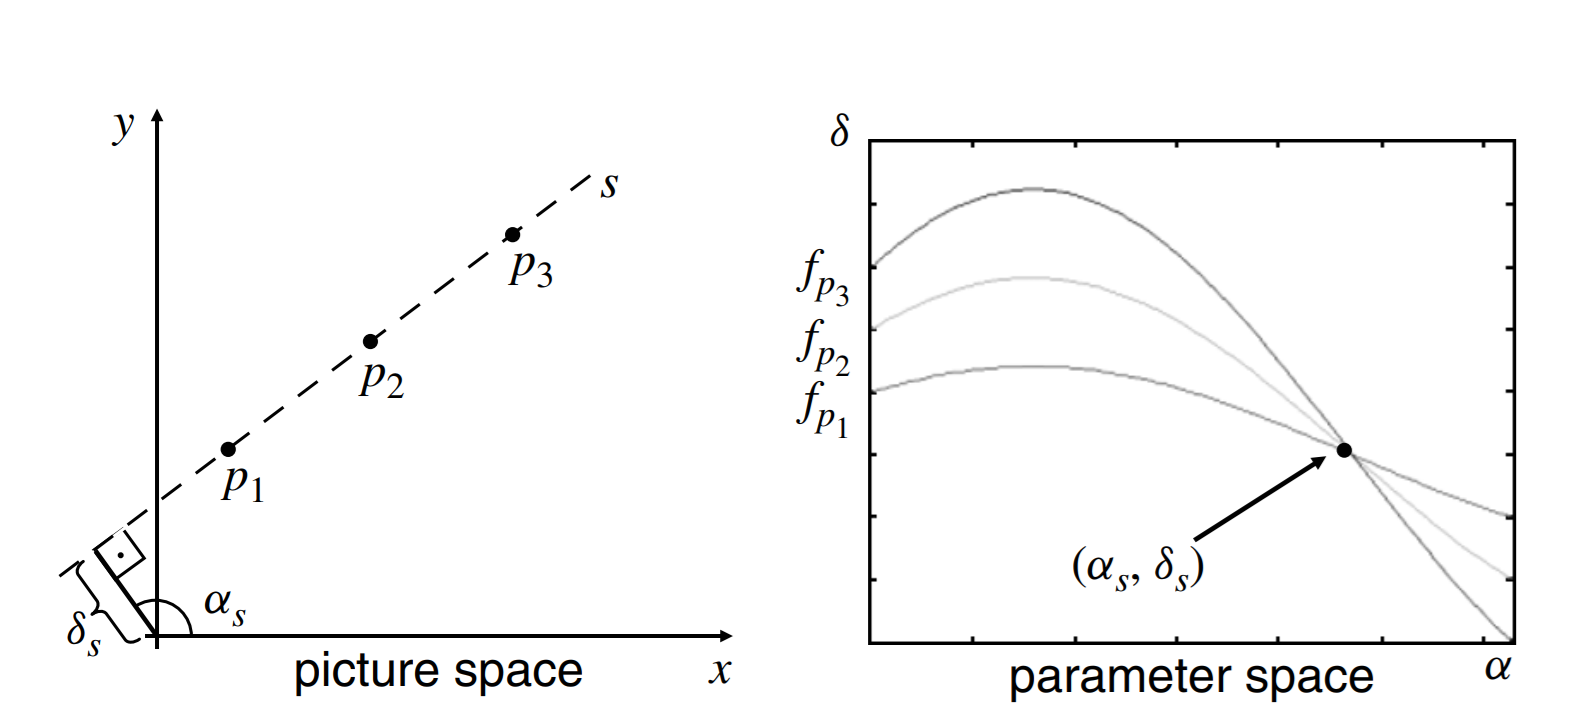
\includegraphics[width=0.9\textwidth]{figures/TODOHOUGHTHETADIST.png}
    \caption{Hough transform into a $(\alpha,\delta)$-parameter space\cite{CASHachtert2008global}.}
    \label{fig:TODOHOUGH}
\end{figure}

Summarized this duality between data and parameter space results in the following properties:\label{ssec:properties}
\todor{choose a style}
\begin{property}\label{prop:hough1}
A point in data space corresponds to a (sinusoidal) function in the parameter space. 
\end{property}
\begin{property}\label{prop:hough2}
A point in parameter space corresponds to a linear function in the data space.
\end{property}
\begin{property}\label{prop:hough3}
Points lying on the same line in data space have a common intersection in parameter space.
\end{property}
\begin{property}\label{prop:hough4}
Points lying on the same (sinusoidal) function in parameter space correspond to lines through the same point in data space.
\end{property}

Since points in parameter space correspond to a linear function in data space and a curve in parameter space corresponds to a point in data space, we can deduct that intersections of curves in parameter space correspond to points lying on the same line in data space. Therefore through the transformation, the problem of finding correlated points becomes a problem of finding points or regions of intersections of curves in parameter space. 
Another added benefit is the parameter space's independence of the locality assumption since regardless of the points' locations in data space its functions' intersections in parameter space represent points lying on the same line. \todor{wtf sentence} 
To solve this problem, there are several approaches. 
For exact results, looking for points with high intersections can be done by solving linear equation systems of the functions in parameter space. 
This, however, can quickly become computationally infeasible and does not cope with jitter, which causes disruptions in the exact intersections in parameter space. 
Static predefined grid-based approaches, like searching for 2-dimensional regions of interest with a predefined grid/accumulator using a voting scheme, or dynamic approaches, like done in \textcite{CASHachtert2008global} by splitting the 2d search space more efficiently, are some computationally less expensive solutions. 
An in-depth explanation of one approach, namely \acrfull{cash}, will be given in the following \fullref{ssec:CASHindepth}.

\subsection{CASH - In Depth}\label{ssec:CASHindepth}
\todo{check n-dim Hough transform explanation with DK}
\acrfull{cash} is a subspace clustering algorithm based on the principle of the Hough transform which, in contrast to the axis-parallel algorithms \acrshort{subclu}\cite{sublcukailing2004density} and \acrshort{clique}\cite{cliqueagrawal1998automatic}, can detect arbitrarily oriented subspaces (c.f.~\autoref{ssec:houghindepth}. \todor{sounds awful}
For arbitrary-dimensional data spaces $\mathcal{D} \subseteq \R^d$ \textcite{CASHachtert2008robust} reformulates the Hough transformation via a generalized description of spherical coordinates. A $d$-dimensional point/vector $x=(x_1,\dotsc,x_d)$ w.r.t.\ the given orthonormal basis $e_1,\dotsc,e_d$, can be described with $d-1$ independent angles $\alpha_1,\dotsc,\alpha_{d-1}$ and the norm/distance to origin of vector/point $x$. The following definitions are taken from \cite{CASHachtert2008robust}:

\subsubsection*{Spherical Coordinates}\label{def:spherecord}
\todor{verbatim definition!}
Let $e_i, 1 \leq i \leq d$, be an orthonormal basis in a $d$-dimensional feature space. Let $x=(x_1,\dotsc,x_d)$ be a $d$-dimensional vector on the hypersphere of radius $r$ with center at the origin. Let $u_i$ be the unit vector in the direction of the projection of $x$ onto the manifold spanned by $e_i,\dotsc,e_d$. For the $d-1$ independent angles $\alpha_1,\dotsc,\alpha_{d-1}$, let $\alpha_i$, $1 \leq i \leq d-1$, be the angle between $u_i$ and $e_i$. Then the generalized spherical coordinates of vector $x$ are defined by:
\begin{align}
    x_i = r \cdot (\prod_{j=1}^{i-1}\sin{\alpha_j}) \cdot \cos{\alpha_i}\text{, where } \alpha_d = 0.
\end{align}

Similar to \autoref{ssec:houghindepth}, any $d$-dimensional point $p \in \mathcal{D}$ can be explained by an infinite number of hyperplanes containing $p$. These hyperplanes can be uniquely defined by the $d-1$ angles $\alpha_1,\dotsc,\alpha_{d-1}$, with $\alpha_i \in [0,\pi)$ representing the normal vector of the hyperplanes, and a fix point $o$ on the hyperplane. To acquire a point independent representation \textcite{CASHachtert2008robust} maps the angles $\alpha_i$ and point $p$ with the following parametrization function to the shortest distance $\delta$ of the hyperplane to the origin (c.f. \ref{eq:hnfangles}).

\subsubsection*{Parametrization Function}
Let $\vec{p} = (p_1,\dotsc,p_d)$ be a $d$-dimensional vector and $\vec{n_0} = (n_1,\dotsc,n_d)$ be a $d$-dimensional unit vector specified by $d-1$ angles $\alpha_1,\dotsc,\alpha_{d-1}$ according to the \hyperref[def:spherecord]{previous definition \textit{``Spherical Coordinates''}}. Then the parametrization function $f_{\vec{p}}:\R^{d-1} \rightarrow \R$ of vector $\vec{p}$ denotes the distance of the hyperplane defined by the point $p$ and the normal vector $\vec{n}$ to the origin:
\begin{align}
    \begin{split}
            f_{\vec{p}}(\alpha_1,\dotsc,\alpha_{d-1}) &= \langle \vec{p},\vec{n_0} \rangle\\
    &= \sum_{i=1}^d p_i \cdot (\prod_{j=1}^{i-1} \sin{\alpha_j}) \cdot \cos{\alpha_i}  = \delta
    \end{split}
\end{align}

Given $d-1$ angles $\alpha_1,\dotsc,\alpha_{d-1}$ and shortest distance $\delta$ obtained by the parametrization function for a point $p_i = (x_1,\dotsc,x_d)$ and its infinite hyperplanes, each point $p$ in data space $\mathcal{D}$ can be mapped to a $d$-dimensional parameter space $\mathcal{P} \subseteq \R^d$ spanned by the previously mentioned parameters, again creating a function defining a hyperplane:
\begin{align}
    \begin{split}
        \delta &= x_1 \cdot n_{0,1} + \dots + x_d \cdot n_{0,d}\\
        &= \langle \vec{x},\vec{n_0} \rangle\label{eq:highhnf}
    \end{split}
\end{align}

Similar to \autoref{ssec:houghindepth} the resulting hyperplane in parameter space can be transformed between  cartesian representation using a unit vector $\vec{n_0}$ and polar representation based on angles $\alpha_1,\dotsc,\alpha_{d-1}$. In the process of this thesis, we primarily use the cartesian form of the \gls{hnf} (c.f. \autoref{eq:highhnf}).


By the means of the parametrization function \textcite{CASHachtert2008robust} extend the properties of the original Hough transformation (c.f. \autoref{ssec:properties}) to $d$-dimensional data spaces and its corresponding parameter spaces: \todor{verbatim}
\begin{quoting}
\begin{property}
A point $p$ in data space $\mathcal{D} \subseteq \R^d$ is represented by a sinusoidal curve $f_p:\R^{d-1}\rightarrow\R$ in parameter space.
\end{property}
\begin{property}
A point $p' = (\alpha_1,\dotsc,\alpha_{d-1},\delta$ in parameter space $\mathcal{P} \subseteq R^d$ corresponds to a $(d-1)$-dimensional hyperplane in data space.
\end{property}
\begin{property}
Points that are located on a $(d-1)$-dimensional hyperplane in data space correspond to sinusoidal curves through a common point in parameter space.
\end{property}
\begin{property}
Points lying on the same sinusoidal curve in parameter space represent $(d-1)$-dimensional hyperplanes through the same point in data space.
\end{property}
\end{quoting}

% \begin{enumerate}
%     \item A point $p$ in data space $\mathcal{D} \subseteq \R^d$ is represented by a sinusoidal curve $f_p:\R^{d-1}\rightarrow\R$ in parameter space.
%     \item A point $p' = (\alpha_1,\dotsc,\alpha_{d-1},\delta$ in parameter space $\mathcal{P} \subseteq R^d$ corresponds to a $(d-1)$-dimensional hyperplane in data space.
%     \item Points that are located on a $(d-1)$-dimensional hyperplane in data space correspond to sinusoidal curves through a common point in parameter space.
%     \item Points lying on the same sinusoidal curve in parameter space represent $(d-1)$-dimensional hyperplanes through the same point in data space.
% \end{enumerate}
\missingfigure[]{3d example, fig anfragen}
\begin{figure}
    \centering
    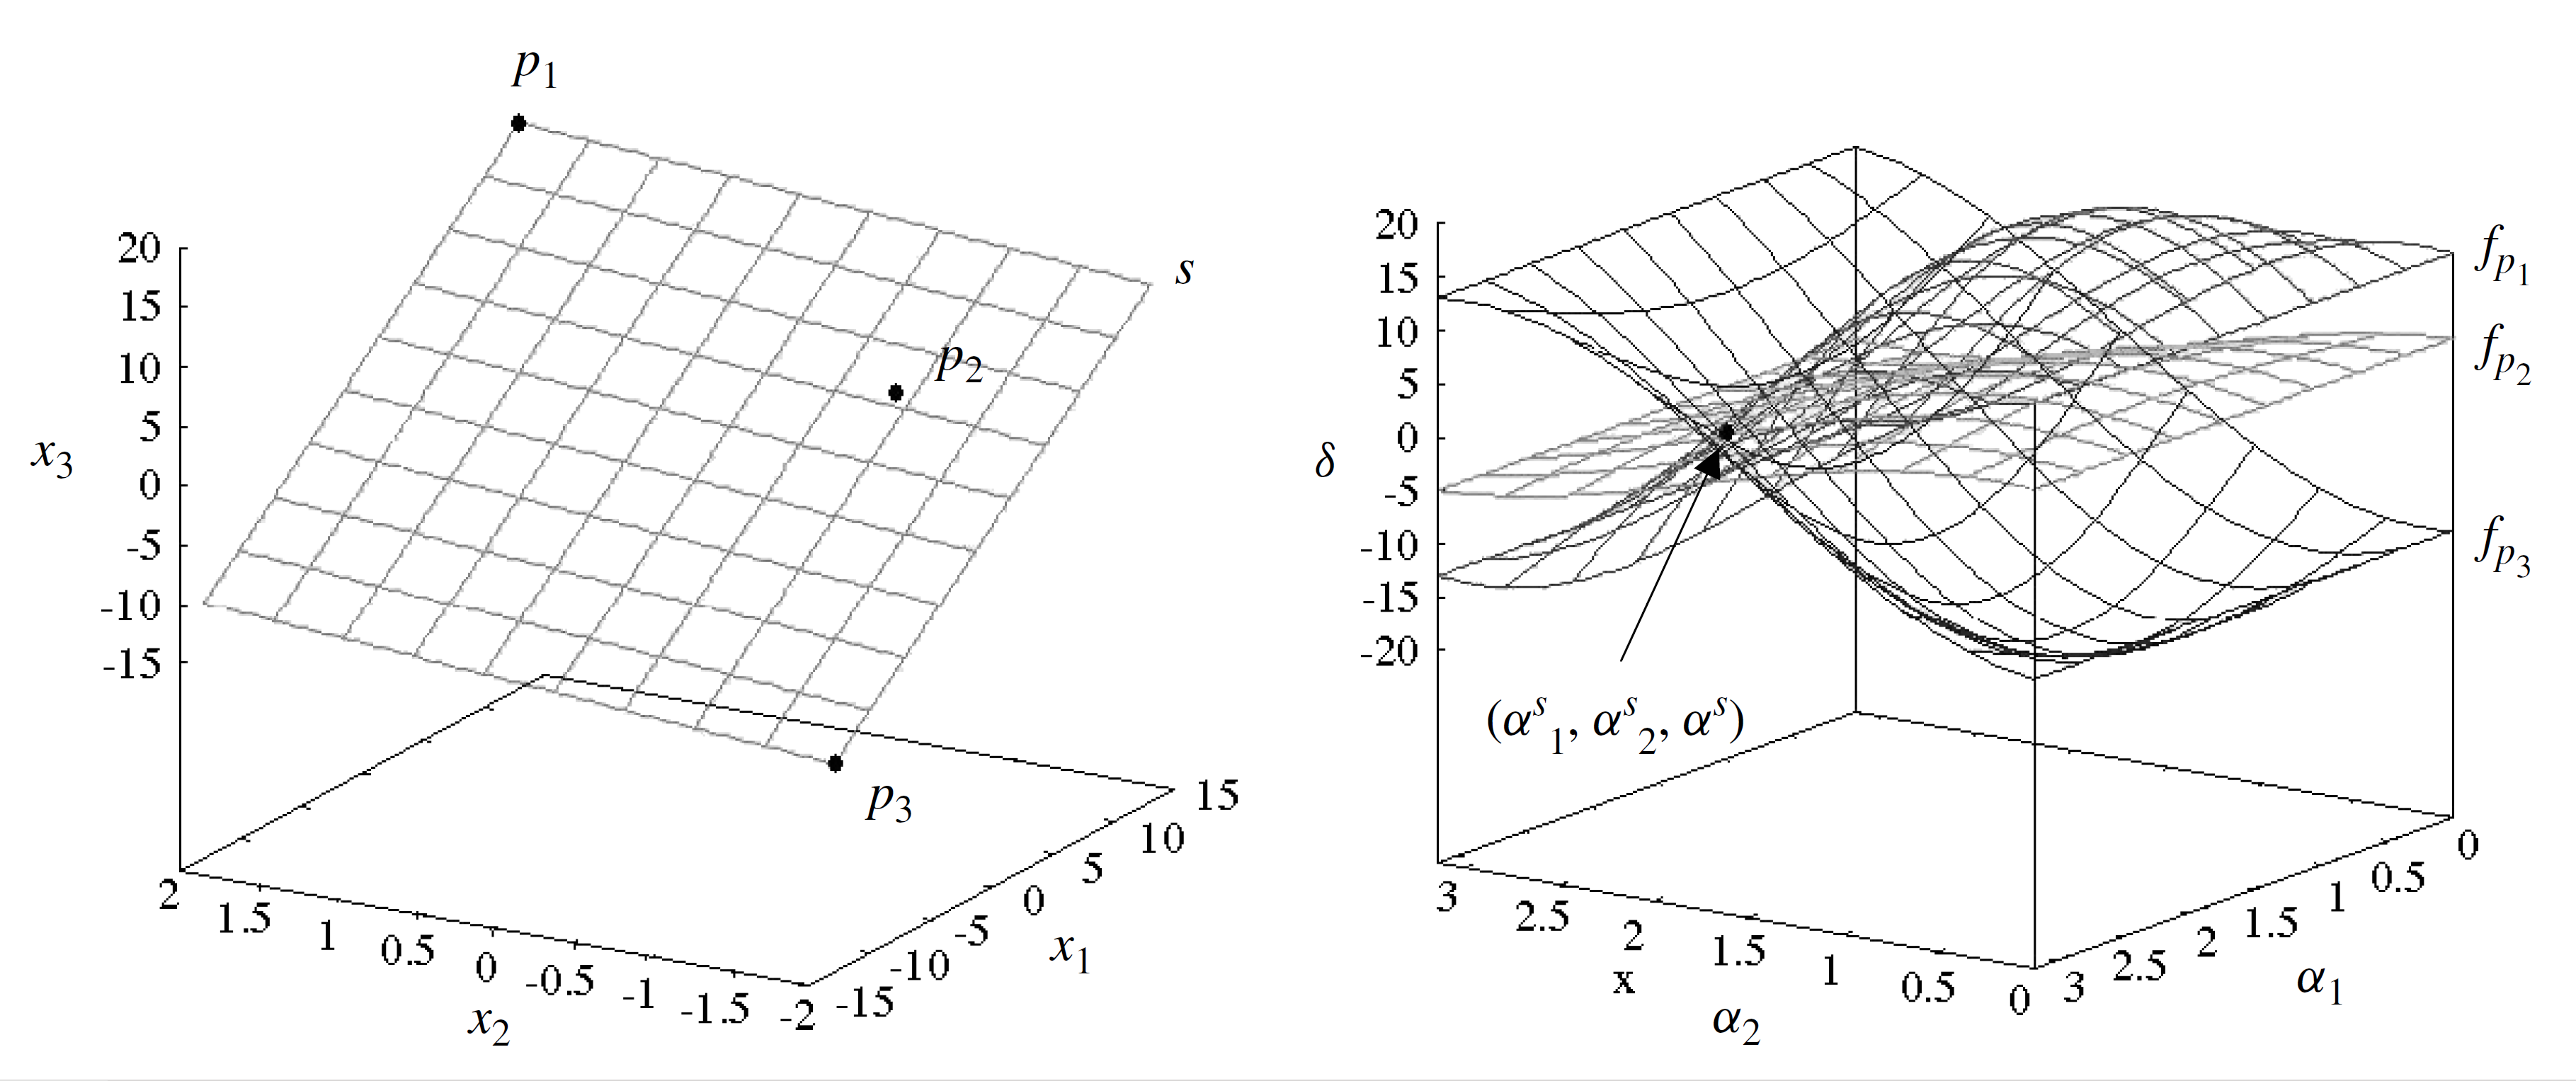
\includegraphics[width=0.9\textwidth]{figures/cash3d.png}
    \caption{Hough transform of a 3-dimensional space creates sinusoidal curves~\cite{opticsankerst1999optics}.}
    \label{fig:cash3d}
\end{figure}

The boundaries of the parameter space $\mathcal{P}$ are extended to \begin{align}
    \mathcal{P} = [\delta_{min}, \delta_{max}]\times [0,\pi)^{d-1}
\end{align} with $\delta_{min}$ and $\delta_{max}$ being the minimum and maximum of all functions $f_p$ for $\alpha \in [0,\pi)$ again: 
\begin{align}
    [\delta_{min}, \delta_{max}] = [min_{p \in \mathcal{D}}(f_p(\alpha_p^{min})), max_{p \in \mathcal{D}}(f_p(\alpha_p^{max}))]
\end{align} 
where $\alpha_p^{min}$ and $\alpha_p^{max}$ denote the minimum and maximum of function $f_p$. An in detail explanation is found in \textcite{CASHachtert2008robust}.
Applying the same concept of \autoref{ssec:houghindepth} the goal of finding $d$-dimensional points lying on the same hyperplane requires finding intersections of the corresponding $d$-dimensional curves in parameter space. Since an analytical solution of the intersections in multi-dimensional space is infeasible, the parameter space is scanned for $d$-dimensional regions/hypercuboids of a certain amount $m$ of intersections instead which additionally copes with jitter. Regions which fulfil the number of intersections are called \textit{dense grid cells}.

\subsubsection*{Correlation Cluster}\todor{check definition with dk}
Since we have to distinguish correlation clusters from density-based clusters, we hereby propose a notion of correlation clusters.

Correlation in a classical sense is a measure of relationship between two variables/features, but can also be extended to relations between multiple features. Commonly the relation refers to a linear relationship, but can also be non-linear. Since we want to cluster these correlations not only by orientation, but also by positioning, we define a specifically located correlation $r_{l,f,t}$, with $l$ being an unambiguous location as the source of the correlation, $f$ being a set of predictor features and $t$ being the target/correlating feature, as a hyperplane $h(t,f,l)$. In case of \gls{cash} a localized correlation/hyperplane is defined by the \gls{hnf}(c.f. \autoref{eq:highhnf}) with $f$ and $t$ being embedded in the orientation $n_{0,i} \in \{f,t\}$ and distance $\delta$ and $l$ only being embedded in the latter one. 
\begin{align}
    \delta(t,f,l) = \langle \vec{x},\vec{n_0}(f,t) \rangle
\end{align}

\textit{Correlation clusters} refer to the grouping of observations/data objects within a certain interval in data space which display similar correlations in a subset of the object's features. In other words, a Correlation cluster is a group of points which have a low distance $j$, which we will refer to as \textit{jitter}, to a hyperplane $h$ modelled by a correlation within an interval. We formalize it as following:

A correlation cluster in data set $DS$ is a non-empty subset $C^{Corr} \subseteq DS$ of points $p$ which fulfil the following condition:
\begin{align}\label{eq:pointtohyplane}
    &\forall p: \text{if } \text{dist}(p,h) < j \text{, then } p \in C^{Corr}
\end{align}
where the function $dist(a,b)$ denotes the shortest distance between two geometric objects, $h$ being the hyperplane modeling the localized correlation and $j$ the jitter representing the maximal threshold for fault tolerance. \todor{richtiger begriff dafuer?}

\todor{eigene definition, consistent with dbscan}

\subsubsection*{Correlation Noise}
Analogous to density-based noise in \autoref{ssec:DBSCANindepth}, every point not belonging to any of the existing clusters $C^{Corr}_1, \dotsc, C^{Corr}_k$ in data set $DS$ are now considered noise: 
\begin{align}
    noise^{Corr} = \{p \in  DS | \forall i : p \notin C^{Corr}_i\}
\end{align}

\subsubsection*{The CASH-Algorithm}
Given previously defined data representation in data and parameter space, the goal is finding dense grid cells in parameter space. However, since the complexity of searching the parameter space with a predefined grid is exponential w.r.t.\ dimension $d$, it also quickly gets too computationally expensive for higher dimensional spaces. \gls{cash} tackles this problem by smartly dividing the search space. \citeauthor{CASHachtert2008robust} proposed the following search strategy:
\vspace{5mm}

The parameter space is successively divided by the axes in the static order given by $\delta,\alpha_1,\dotsc,\alpha_{d-1}$. After each split, the hypercuboid with more intersections is divided at the next axis of the order. If both hypercuboids have the same amount of intersections, the first hypercuboid is selected (arbitrarily). The other hypercuboid is kept in a queue, which is ordered descendingly by the number of its intersecting curves/points. If regions in the queue have an equal amount of intersections, the smaller region is preferred. These splits and additions to the queue are done until both split hypercuboids have less than a minimum number of intersections $m$ to be considered dense or a predefined depth $s$ has been reached. If and only if a hypercuboid at split $s$ fulfils $m$, the hypercuboid is considered a valid subspace cluster.
All valid $(d-1)$-dimensional subspace clusters are then recursively re-evaluated by \gls{cash} until the resulting found subspace clusters have a minimum dimensionality of $minDims$. If a subspace cluster is found, its intersecting curves are removed from any other hypercuboid in the queue, which is then updated and sorted according to its new status. If the number of intersections drops below $m$, the hypercuboid is removed from the queue. This procedure is done until the queue is empty.

\vspace{5mm}
\begin{algorithm}[H]
% \algsetup{linenosize=\tiny}
% \scriptsize
\SetAlgoLined
\KwData{parameter space $\mathcal{P}$; queue $Q$ ordered by number of intersections and its volume; iterator $I$ of order of axis $[\delta,\alpha_1,\dotsc,\alpha_{d-1}]$; set of subspace clusters $C$; minimum number of intersections $m$; maximum number of splits $s$}
\KwResult{Set of clusters $C$ representing the subspaces found in $\PS$}
\SetKwFunction{CASH}{CASH}
\SetKwProg{Fn}{Function}{:}{\KwRet $C$}
Q := $\emptyset$\;     
h1 := first hypercuboid of split\;
h2 := second hypercuboid of split\;
h := $\PS$\tcp*{working hypercuboid}
\Fn{\CASH{$h$, $m$, $s$}}{
     \Do{$Q$ is not empty}{
        h1, h2 := h.splitAxis($I$.next())\;
        h := $arg\,max_{cube \in \{h1,h2\}}(cube.intersections)$\;
        Q.add(\{h1,h2\}$\setminus$ h)\;
        splitcounter := 1\;
        \While{$h.intersections > m$ and $splitcounter < s$}{
            h1, h2 := h.splitAxis($I$.next())\;
            splitcounter++\;
            h := $arg\,max_{cube \in \{h1,h2\}}(cube.intersections)$\;
            Q.add(\{h1,h2\}$\setminus$ h)\;
        }
        \If{$h.intersections > m$}{
            $C := C\ \cup$\ \CASH{h,m,s}\;
        }
        $I$.reset()\tcp*{reset Iterator for split of next $h$}
        $Q$.removeIntersectionsAndUpdate($C$)\;
    }
}

 \caption{CASH}
\end{algorithm}
\vspace{5mm}

All things considered, the average time complexity of \gls{cash} condenses to $\mathcal{O}(s \cdot c \cdot |DS| \cdot d^3)$, where $s$, $DS$ and $d$ are as previously mentioned and $c$ denotes the number of clusters in $DS$, however in the worst case scenario, where every point is in the deepest cell, the complexity rises to $\mathcal{O}(2^d)$. The resulting set $C$ contains all $n$-dimensional subspace clusters with $n < d$ found within the constraints of minimum points in correlation $m$ and maximum splits $s$.\\
\todor{Check recursive CASH}

We now possess the means to find density-based clusters and global subspace clusters in an original data set $DS$. The density-based approach \gls{optics} requires two parameters, a minimum number of points $minPts$ and a maximum epsilon distance $\epsilon$, which essentially specify the minimum density allowed, to acquire a hierarchical view of density-connected clusters in $DS$. The subspace clustering approach \gls{cash} also requires another two parameters, a minimum number of points/intersections $m$ and a number of splits $s$ to be considered a subspace cluster.

\section{The Algorithm}
With the previously mentioned algorithms, we are already able to find arbitrarily shaped clusters with a density-based approach, and arbitrarily oriented subspace clusters with, e.g. \gls{4c} or \gls{cash}, however, all of them are restricted to finding those clusters in a purely local or purely global fashion. E.g. none of the previously mentioned algorithms can handle both scenarios, as shown in \autoref{fig:badscenario}.

% \begin{figure}
%     \centering
%     \begin{minipage}{.47\textwidth}
%       \centering
%       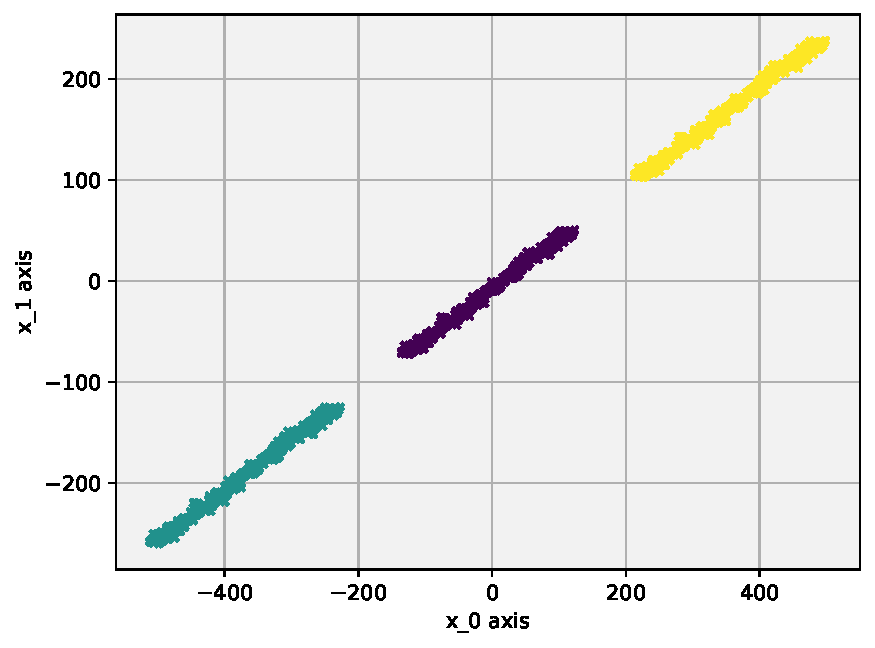
\includegraphics[width=.8\textwidth]{figures_method/piecewisecorrs.pdf}
%       \captionsetup{width=0.8\linewidth}
%       \captionof{figure}{Separated locally dense clusters following a Correlation.}
%       \label{fig:scenario1}
%     \end{minipage}%
%     \begin{minipage}{.47\textwidth}
%       \centering
%       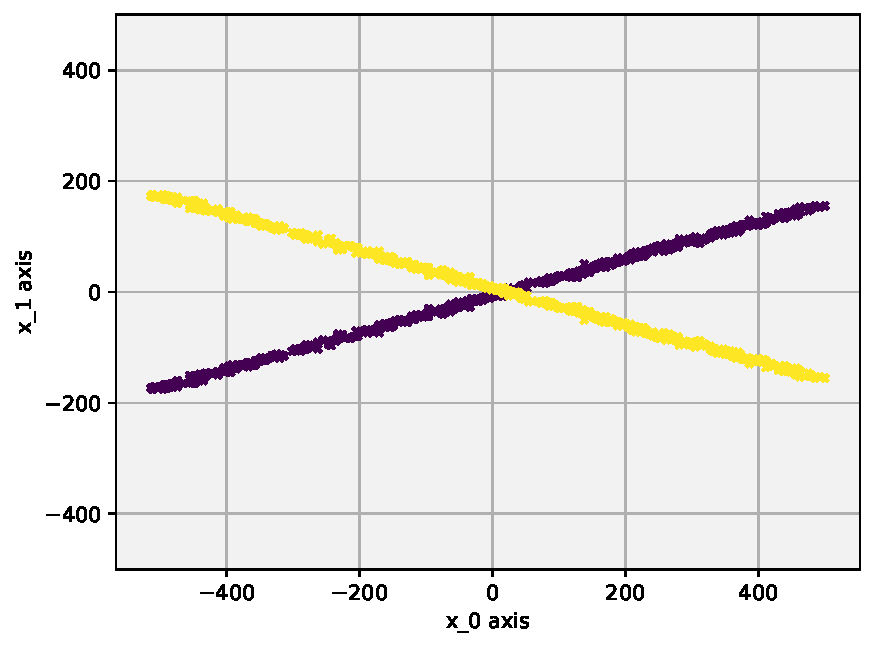
\includegraphics[width=.8\textwidth]{figures_method/xcorrs.pdf}
%       \captionsetup{width=0.8\linewidth}
%       \captionof{figure}{Connected dense clusters following two different Correlations.}
%       \label{fig:scenario2}
%     \end{minipage}
%     \caption{Problemsettings for methods with fixated scope: purely local or purely global.}
%     \label{fig:badscenario}
% \end{figure}

\begin{figure}
    \centering
    \begin{subfigure}[t]{0.47\textwidth}
      \centering
      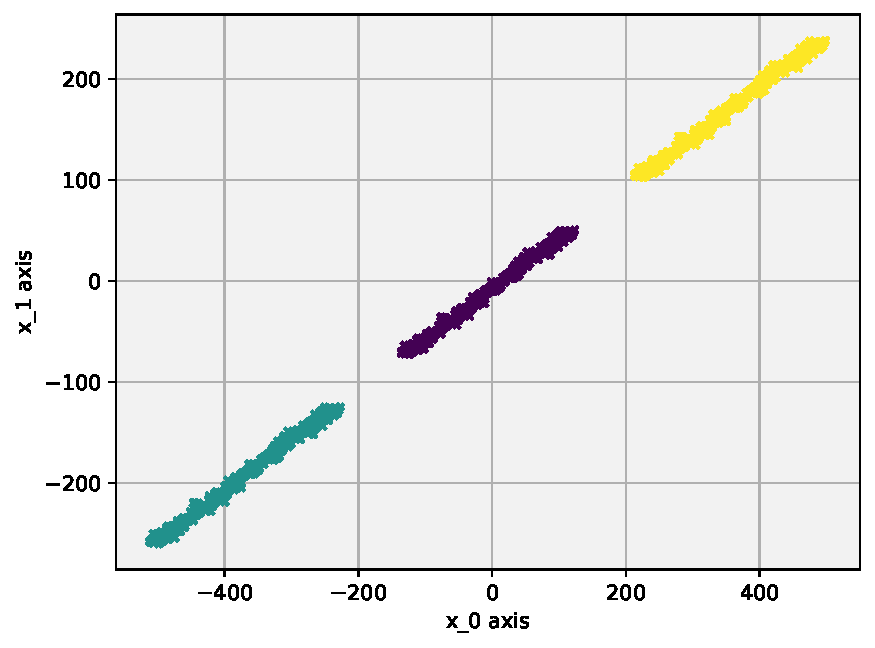
\includegraphics[width=.8\textwidth]{figures_method/piecewisecorrs.pdf}
      \captionsetup{width=0.8\linewidth}
      \caption{Separated locally dense clusters following a Correlation.}
      \label{fig:scenario1}
    \end{subfigure}%
    \begin{subfigure}[t]{0.47\textwidth}
      \centering
      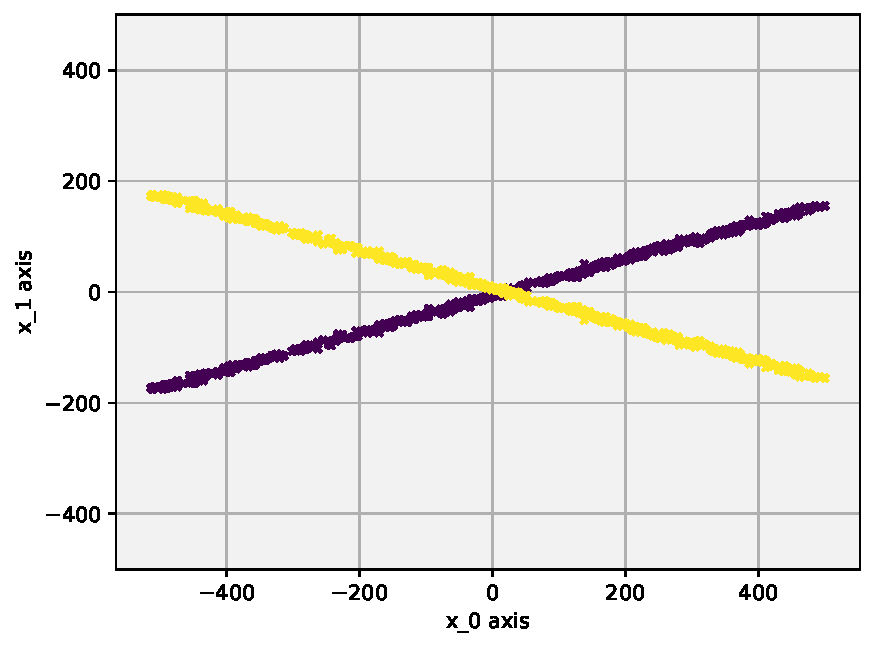
\includegraphics[width=.8\textwidth]{figures_method/xcorrs.pdf}
      \captionsetup{width=0.8\linewidth}
      \caption{Connected dense clusters following two different Correlations.}
      \label{fig:scenario2}
    \end{subfigure}
    \caption{Problem settings for methods with fixated scope: purely local or purely global.}
    \label{fig:badscenario}
\end{figure}

% \begin{figure}
%     \centering
%     \includegraphics{}
%     \missingfigure[]{scenario zeigen}
%     \caption{Caption}
%     \label{fig:scenario}
% \end{figure}
\autoref{fig:scenario1} \todor{figure erstellen} depicts a setting, where the data contains multiple characteristic local correlations which however cannot be accurately described by the aforementioned global methods alone. 
\autoref{fig:scenario2} shows a dense cross-shaped cluster which cannot be separated by \gls{dbscan} or \gls{optics} while additionally not being able to deliver their correlations. 
The extension \gls{4c} is able to detect the local correlations, however can get skewed results in the crosses due to the correlations orientation not being accurately representable by the eigenvectors of the \gls{pca}\cite{PCAshlens2014tutorial}. 
\gls{cash} on the other hand could find the correlations. 

\begin{figure}
    \centering
    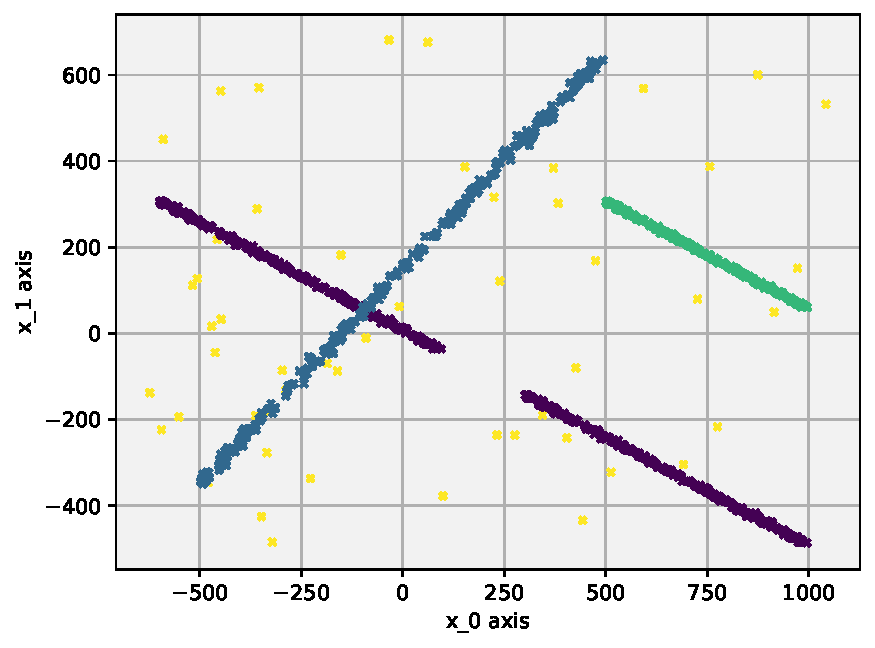
\includegraphics[width=.7\textwidth]{figures_method/Groundtruth.pdf}
    \caption{Example data set $DS$}
    \label{fig:localglobalproblem}
\end{figure}

\autoref{fig:localglobalproblem} \todor{figure} shows multiple local settings of different correlations which neither of the aforementioned methods can solve in a satisfactory manner. \gls{4c} is able to find the accurate local correlations, however, can not categorize those local correlations as one global correlation. 
On the other hand, \gls{cash} can only find the global correlation while omitting the information of the gaps in data. Hierarchical subspace clustering methods like \acrshort{hico} and \acrshort{eric} do not address the problem either, since their hierarchy is also based on global lower-dimensional subspaces contained in the original space and not spaces composed of same dimensional subintervals of the same space. 
These subintervals of a space further will be referred to as \textit{subclusters} or \textit{cluster partitions}\todor{2 begriffe oder lieber consistent einen benutzen?}.
So either the subspace clustering method detects local correlations while missing the big picture or they do find global correlations while losing structural information of its particular correlation. This thesis proposes an algorithm that unifies local and global correlation clustering by evaluating \textit{locally dense} regions of interest with a correlation clustering method, e.g. \gls{cash}, and combining those local intermediate correlations into a global correlation clustering to get a universal subspace clustering result. 

%Additionally it does not categorize both horizontal local correlations as one, even though they arguably could be interpreted that way.
% , not the big picture

\subsection{Partitioning Data into Dense Clusters}\label{ssec:partitioning}
The first step we perform is the partitioning of the data space into dense clusters via a density-based clustering approach like \gls{dbscan} or \gls{optics} to force a localized view for consideration of local feature relevance and to create intermediate local clusters. 
%However like mentioned in \autoref{ssec:DBSCANindepth} and \autoref{ssec:OPTICSindepth}
Since we want to find \textit{local} linear correlations within \textit{global} linear correlations, we assume that the global linear correlation is composed of a set of its local linear correlations. This also means that points belonging to the same global linear correlation are also part of the composing local subclusters which have a similar inherent linear correlation as the global correlation. These subclusters have a continuous distribution of density compared to the global correlation itself since else it would have been split as well and counted as separate local subcluster. Vice versa the local components are also disjunct to each other since else there would be a connection to each other to create a bigger cluster partition. Although it is not optimal even if there is an overlap of different global linear correlations and the cluster partition contains multiple of them, it still can retain the information of its composing linear correlations.
We can, therefore, retrieve these local subclusters by searching the data for density-connected sets of points via a density-based clustering approach like \gls{dbscan} or \gls{optics}. This comes with an additional benefit by automatically removing noise. 

However like mentioned in \autoref{ssec:DBSCANindepth} and \autoref{ssec:OPTICSindepth} \gls{dbscan} is not able to find clusters with different density and mixes multiple densities together into one cluster due to its global parameter setting only defining a minimum density. High variance in data densities can therefore strongly influence the result of \gls{dbscan}, either by making it harder to choose the appropriate parameters for a better clustering result or by having more variety in density in found clusters which would result in less conclusive detection of their linear correlations. 
To receive a more suited clustering, we preferred the use of \gls{optics}, which is able to detect clusters with different densities (c.f.~\autoref{ssec:OPTICSindepth}). Since we do not want to prune any information away, we can generally use a very high epsilon-distance $\epsilon$ to create a detailed ordering and therefore only rely on $MinPts$ as a parameter. From this ordering, we can extract clusters with a new parameter $reachdist_{\tau}$ which represents the threshold at which the difference of neighbouring reachability-distances of the ordering is considered to be a new cluster with different density. We also assign a bounding box for each found cluster, which represents the local data space for further evaluation performed by \gls{cash}. As previously mentioned, our density-based methods suffer from the \textit{Curse of Dimensionality}. However, this property at least should not greatly impact the global correlation clustering result, since, if every point has a too sparse neighbourhood, every point would be considered noise and a default \gls{cash} would be applied onto the whole data set. Up to this point, we are merely partitioning the data into dense clusters with the added benefit of filtering out $noise^{DB}$ points (noise points in a density-based view). We will reconsider those noise points later since they still could be parts of the global correlation clustering despite not being dense. \autoref{fig:boundingbox} visualizes a data set after step 1 is performed. The relevant part of the data set is clustered by density, and the bounding boxes highlight its boundaries.

\begin{figure}[h]
    \centering
    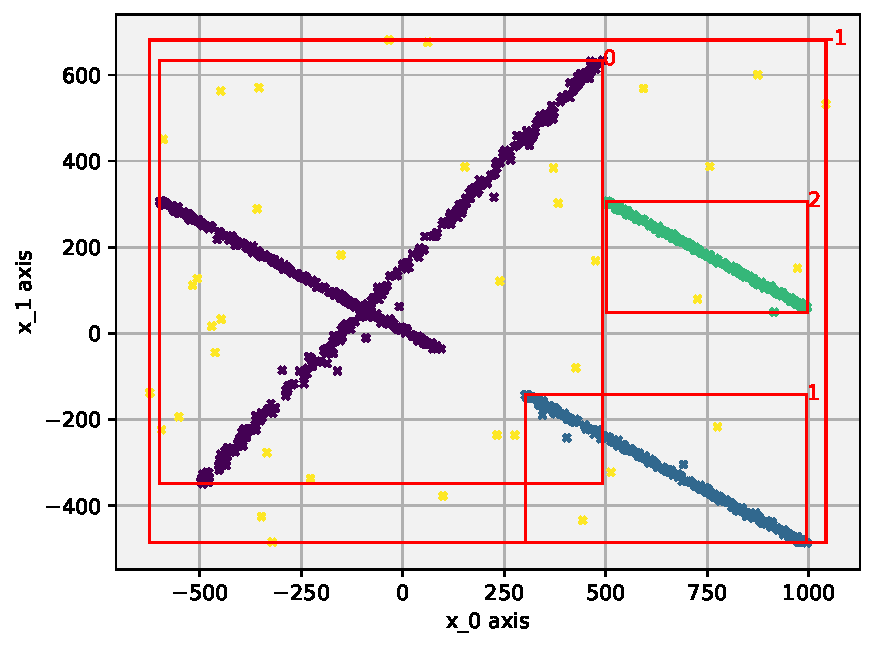
\includegraphics[width=.7\textwidth]{figure_method_grid/DSwithBoundingBoxes.pdf}
    \caption{$DS$ processed by \acrshort{dbscan}, red boxes denote the intervals of the locally dense cluster.}
    \label{fig:boundingbox}
\end{figure}

\subsection{Finding Local Linear Correlations}\label{ssec:findinglocals}
Based on the assumption that local linear correlations contained in a global linear correlation have similar orientations as their parents\todor{parent richtiger begriff?}, we extract all correlations of the dense clusters with a subspace clustering method and in a later step combine them and rebuild the global correlation clustering. 
The second step, therefore, is the extraction of all local linear correlations of all dense clusters within their respective bounding boxes in data space. Since we only consider the points of the locally dense subclusters without/less noise, we can use a variety of methods to extract the linear correlations via global subspace clustering algorithms. 

\begin{figure}[h]
    \centering
    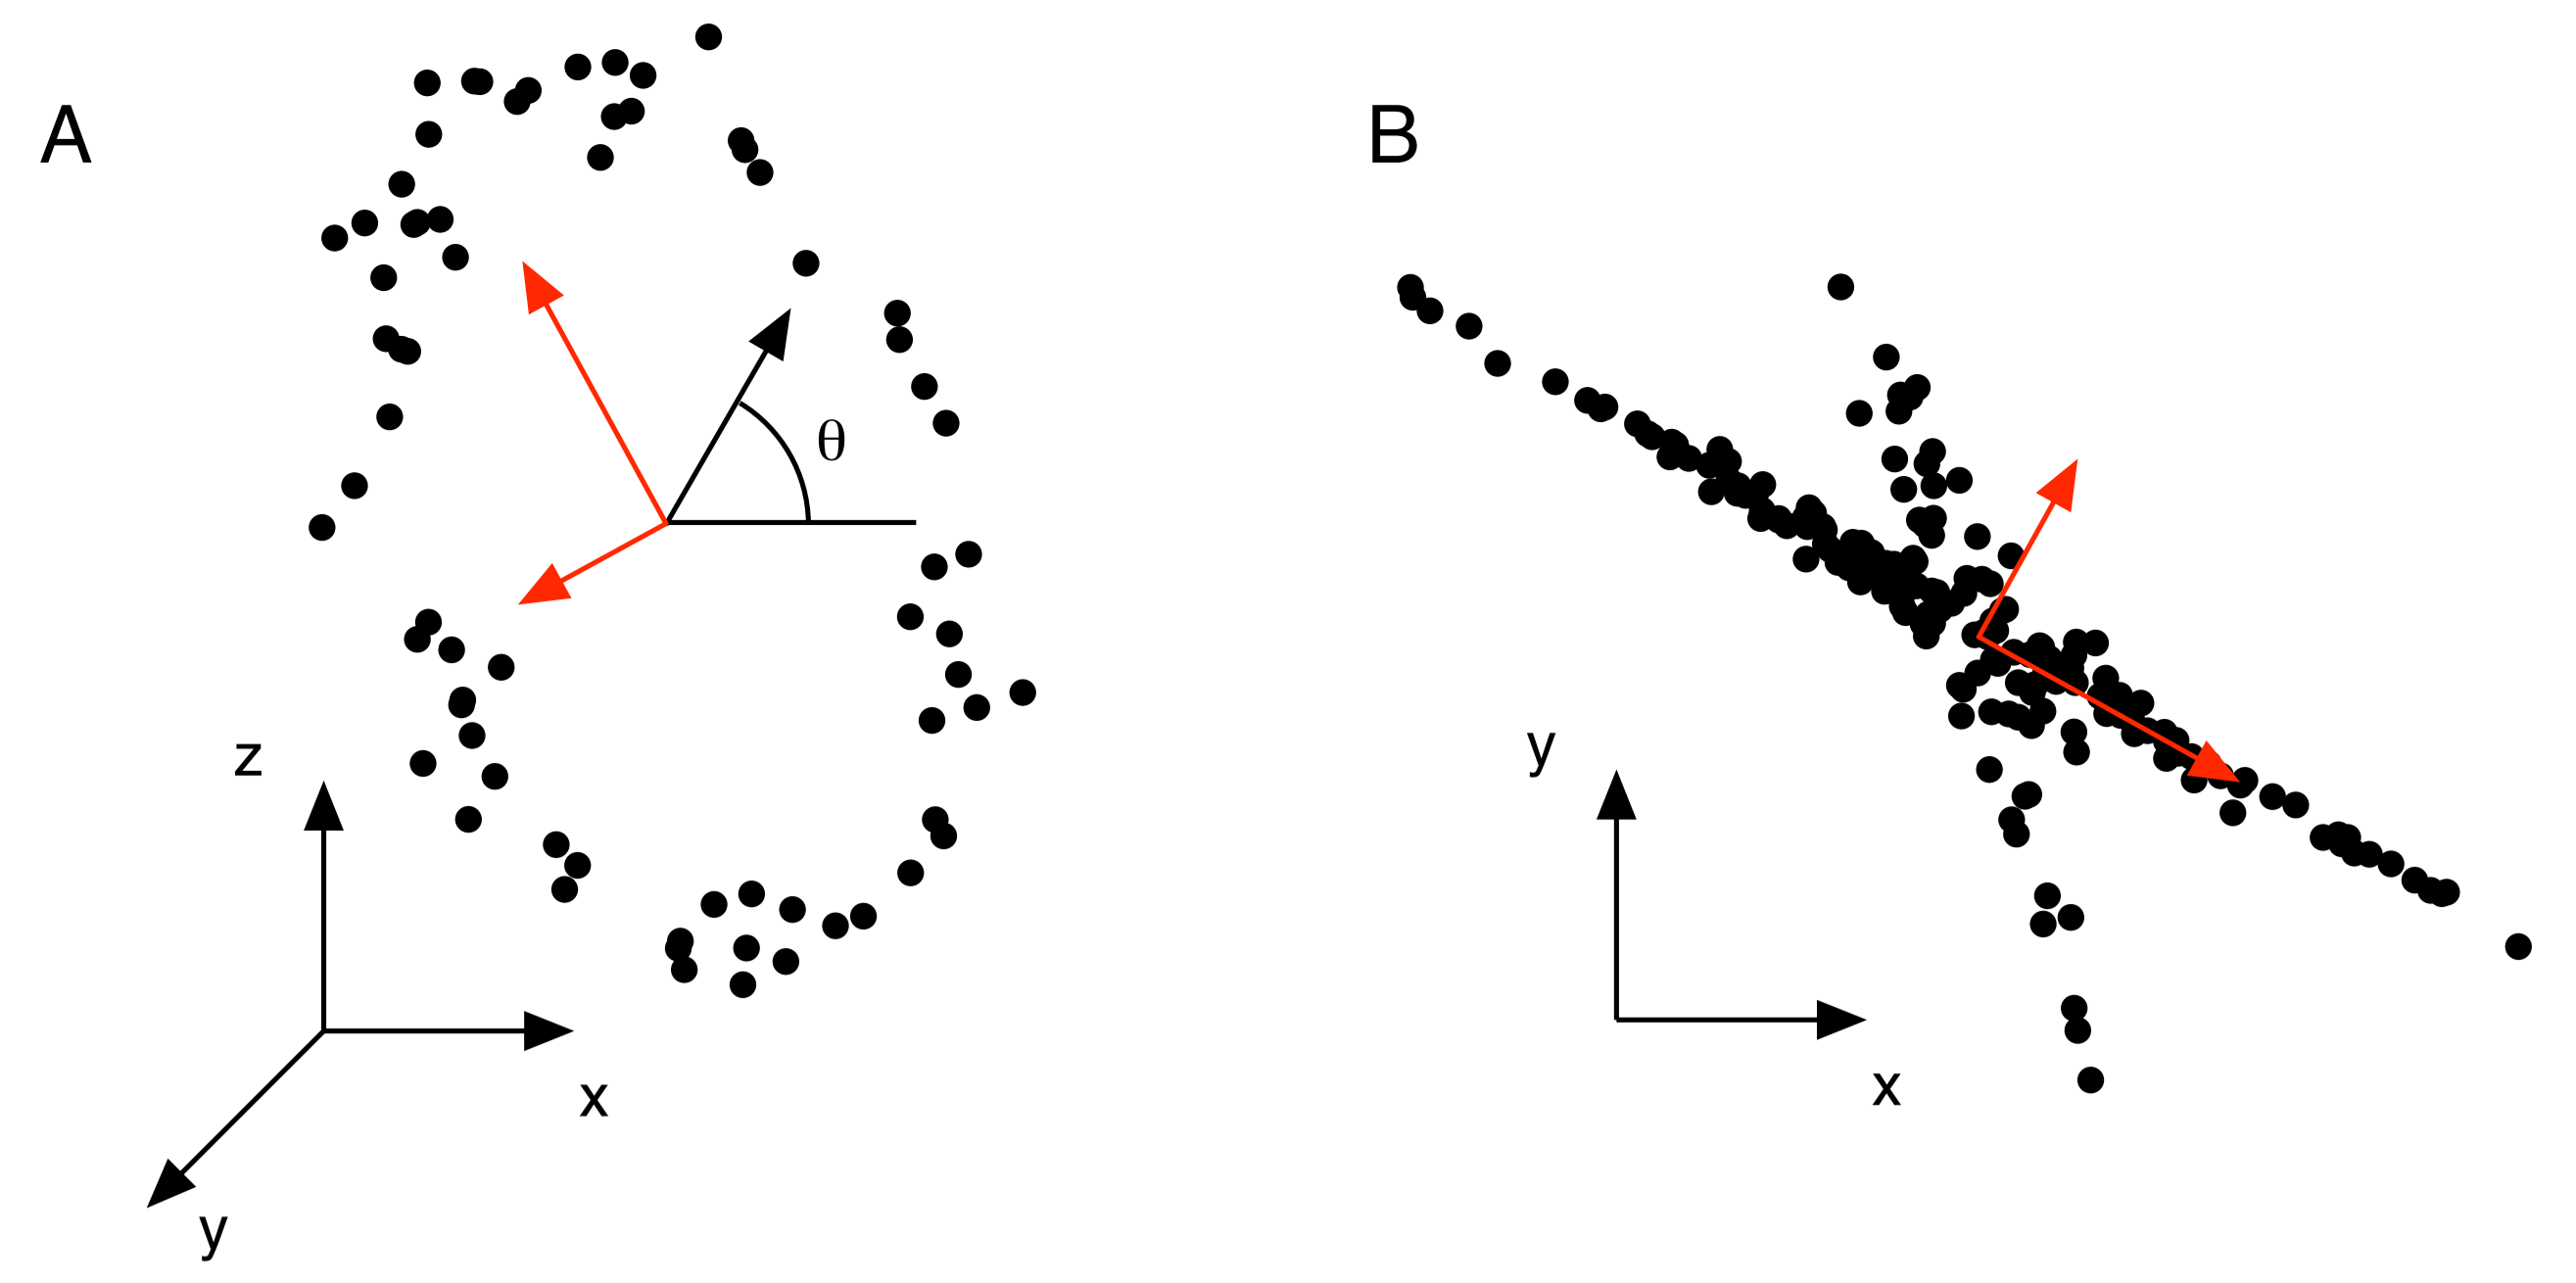
\includegraphics[width=0.8\textwidth]{figures/PCAdifficulties.png}
    \caption{Difficulties for pure \acrshort{pca} to detect all intrinsic Correlations~\cite{PCAshlens2014tutorial}.}
    \label{fig:pcadifficulties}
\end{figure}

To be able to get accurate results, a \gls{pca} would be sufficient if the dense subclusters had either only a single linear correlation or almost orthogonal ones. However, the density-based clustering in step 1 cannot guarantee this property since it can detect arbitrary shapes. This means that there could be constellations of points which would heavily skew the results of \gls{pca} (c.f.~\autoref{fig:pcadifficulties})\cite{PCAshlens2014tutorial}. 

Since \gls{4c} is basically looking for dense clusters with a biased distance function first and then applying \gls{pca} it has the same disadvantages as \gls{pca} itself~\cite{4cbohm2004computing}. Our entire subcluster already is defined as dense by the previous step, and therefore \gls{4c} is prone to also label the whole subcluster as (correlation) dense too and to just consider the whole subcluster as its target. Hence applying \gls{pca} afterwards equals to the application of only \gls{pca} onto the whole subcluster. 
\gls{orclus} is also not suited well. It performs a $k$-means like approach first to partition the subcluster~\cite{orclusaggarwal2000finding}, however since our density-based preprocessing step finds different arbitrary shapes, which implies a different number of correlations, in each cluster partition, choosing a meaningful $k$ is difficult or impossible. \todor{soll der teil in related work? Moechte den als uebergang benutzen um die Verwendung von CASH zu begruenden}
Compared to \gls{orclus} and \gls{4c}, \gls{copac} has better capabilities of finding correlation clusters but lacks in the ability to find a generalized view, e.g. it would not identify two intersecting lines in a 3-dimensional space as a possible hyperplane, but as two lines. 

To cover this scenario as well, we choose to adopt \gls{cash}, which does not rely on the clusters' eigenvectors, is resistant to noise and outliers, and creates an accurate view of a subspace with a requested dimensionality.

After finding all dense regions of interest, the subclusters are independently evaluated for their local correlations without considering the other points in data space. 
The extraction of the correlation is realized by applying the \gls{cash} algorithm onto the locally dense clusters. 
\gls{cash} transforms each point of the cluster into the parameter space and splits it according to its parameters minimum Points $m$ and number of splits $s$ as discussed in \autoref{ssec:CASHindepth}. 
The resulting correlations $l_i \in C^{local}$ and their points are then bounded by the region of interests' intervals (bounding box), which represent the local subspace clusters in the dense region.

\begin{figure}
    \centering
    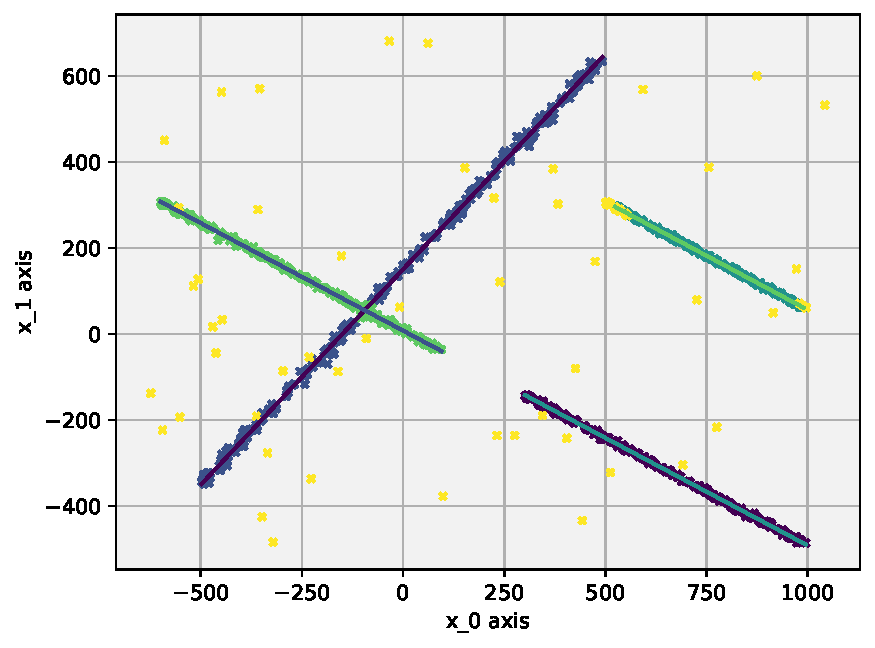
\includegraphics[width=.7\textwidth]{figure_method_grid/LocalLinearCorrelationsWithColoredCorrs.pdf}
    \caption{Intermediate result of the evaluation for Correlations within each locally dense cluster. This represents the local correlation clustering.}
    \label{fig:local_lincorr}
\end{figure}

\subsection{Stitching}\label{ssec:stitching}

To combine the found localized correlations to a global correlation clustering, we evaluate all the localized correlations without their bounding boxes. Since we can represent the localized correlations as hyperplanes with a unit normal vector $\vec{n}$ and a shortest distance to origin $\delta$ (c.f. \autoref{eq:highhnf}), we can easily compare different hyperplanes by variation in rotation (angles), using the cosine-similarity between the normal vectors, and translation (absolute positioning), using the euclidean-distance between the shortest distances. For adjustability we introduce two parameters
$
% \tau_{\Delta \text{cos-dist}}, 
\tau_{\Delta \text{cos-dist}} \in [0,1]$ 
and 
$
% \tau_{\Delta \text{eucl-dist}}, 
\tau_{\Delta \text{eucl-dist}} \in \N$, which serve as thresholds for maximal allowed divergence of both measures. To formalize the requirements for a successful combination (\textit{stitching}) of local correlations we introduce the following relations:\todor{definitionen einfuehren oder textuell einfach beschreiben?}

\subsubsection*{Orientation-Similarity}
Given a set of unique linear correlations $C$ in \gls{hnf}. Then two correlations $c_{a,\delta_a} \in C$ and $c_{b,\delta_b} \in C$ are \textit{orientation-similar}, if the absolute cosine-similarity between the correlations' normal vectors $a$ and $b$ is bigger than $1 - \tau_{\Delta \text{cos-dist}}$.
\begin{align}\label{eq:cosdist}
    |\text{cos-sim}(a,b)| = \left|\frac{\sum_{i=1}^{n} a_{i} b_{i}}{\sqrt{\sum_{i=1}^{n} a_{i}^{2}} \sqrt{\sum_{i=1}^{n} b_{i}^{2}}}\right| > 1 - \tau_{\Delta \text{cos-dist}}
\end{align}

\subsubsection*{Translation-Similarity}
Given a set of unique linear correlations $C$ in \gls{hnf}. Then two correlations $c_{a,\delta_a} \in C$ and $c_{b,\delta_b} \in C$ are \textit{translation-similar}, if the \textit{Orientation-Similarity} holds and the absolute euclidean-distance between the correlations' distances $\delta_a$ and $\delta_b$ is smaller than $\tau_{\Delta \text{eucl-dist}}$.
%  if orientation-similarity (c.f. \autoref{eq:cosdist}) holds and
\begin{align}\label{eq:eucldist}
    |\text{eucl-dist}(\delta_a,\delta_b)| < \tau_{\Delta \text{eucl-dist}}
\end{align}

Given an indexed set of correlations $C=\{c_1,\dotsc,c_n\}$ we define the binary relations for orientation-similarity and translation-similarity as follows:
\begin{align}
    R^{o}=\{\{x,y\} \in C \times C\: \big|\: |\text{cos-sim}(x,y)| > 1-\tau_{\Delta \text{cos-dist}}\}\\
    R^{t}=\{\{x,y\} \in C \times C\: \big|\: |\text{eucl-dist}(x,y)| < \tau_{\Delta \text{eucl-dist}}\}
\end{align}

Using these relations, logical matrices, based on the indexed set of correlations, are created. These matrices serve as filters/masks to model the correlations and their pairwise relations as undirected graphs. Both can, therefore, be interpreted as an adjacency matrix of the correlations.
\begin{align}
    M^{orientation}_{i,j} = 
    \begin{cases}
        1 &\text{ if } (c_i,c_j) \in R^o\\
        0 &\text{ otherwise}
    \end{cases}, \textbf{\quad}
    M^{translation}_{i,j} = 
    \begin{cases}
        1 &\text{ if } (c_i,c_j) \in R^t\\
        0 &\text{ otherwise}
    \end{cases}
\end{align}

To check for similar correlations, we now consider the logical matrices $M^{orientation}$ and/or $M^{translation}$ as a criterion for stitching by applying them, via element-wise product, onto an all-ones matrix, where the element at row $i$ and column $j$ represents the relation between correlation $c_i$ and $c_j$, resulting in the adjacency matrix $A$. 

The connected components of $A$ now represent the set of localized correlations fulfilling previously chosen similarities and are combined into global correlation clusters by applying different average measures of the components, e.g. mean and median. The new global correlation $g$ of a set of connected correlations $S=\{s_1,\dotsc, s_m\}$ is defined as:
\begin{gather}
    \begin{split}
        \vec{S} = \{\vec{n_{s_1}},\dotsc,\vec{n_{s_m}}\}\\
        \delta_S = \{\delta_{s_1},\dotsc,\delta_{s_m}\}\\
        \vec{n}_g = f_{avg}(\vec{S})\\
        \delta_g = f_{avg}(\delta_S)
    \end{split}\\
    \nonumber\\
    \text{hyperplane $g$: } \delta_g = \langle \vec{n}_g, \vec{x}\rangle
\end{gather}
where the function $f_{avg}(X)$ is a user-defined average function over set $X$. Each point previously assigned to one of the components correlation now additionally is labelled with its superordinate global correlation cluster $g_i \in C^{global}$.

\begin{figure}[h]
    \centering
    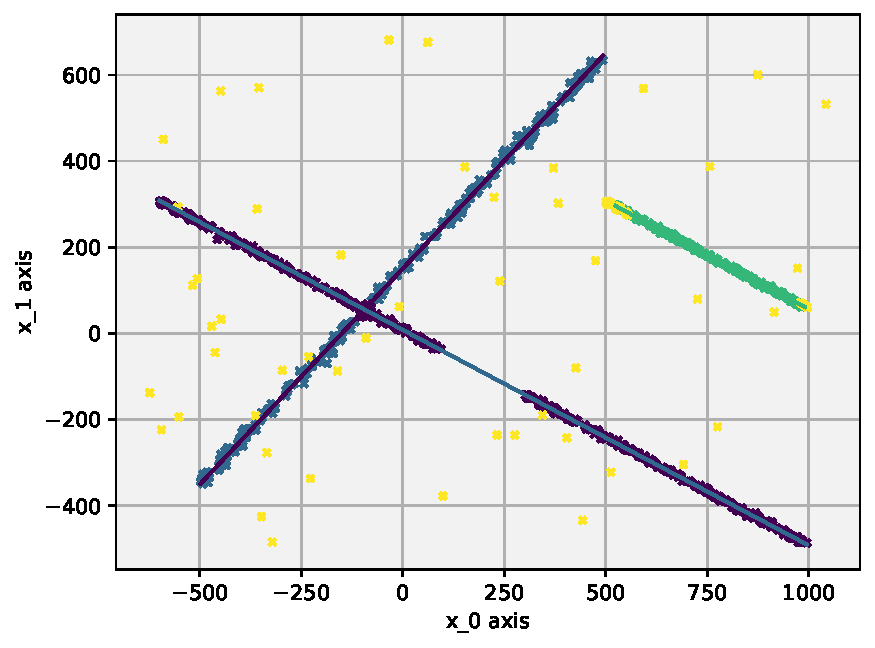
\includegraphics[width=.7\textwidth]{figure_method_grid/StitchedLinearCorrelationsWithColoredCorrs.pdf}
    \caption{Stitching: Similar Correlations are grouped together to form a pseudo-global view.}
    \label{fig:stitchedcorr}
\end{figure}

\subsection{Relabelling}

Since we previously discarded $noise^{DB}$ and $noise^{Corr}$, which were labelled as noise points in a localized view, we now focus on/re-evaluate the membership of those points with regards to the newly created global correlation clusters. 

$Noise^{Corr}$ could have been a member from a far away localized correlation cluster and $noise^{DB}$ was filtered out even before consideration of correlation cluster membership. Hence re-evaluating these points with a global view again complements the result for completeness. This is done by reassessing the distance of all noise points $noise^{DS \cup Corr}$ to all found correlations $C^{local \cup global}$ and relabelling them, if the threshold condition $j$ is fulfilled (c.f. \autoref{eq:pointtohyplane}).\\
\begin{figure}[h]
    \centering
    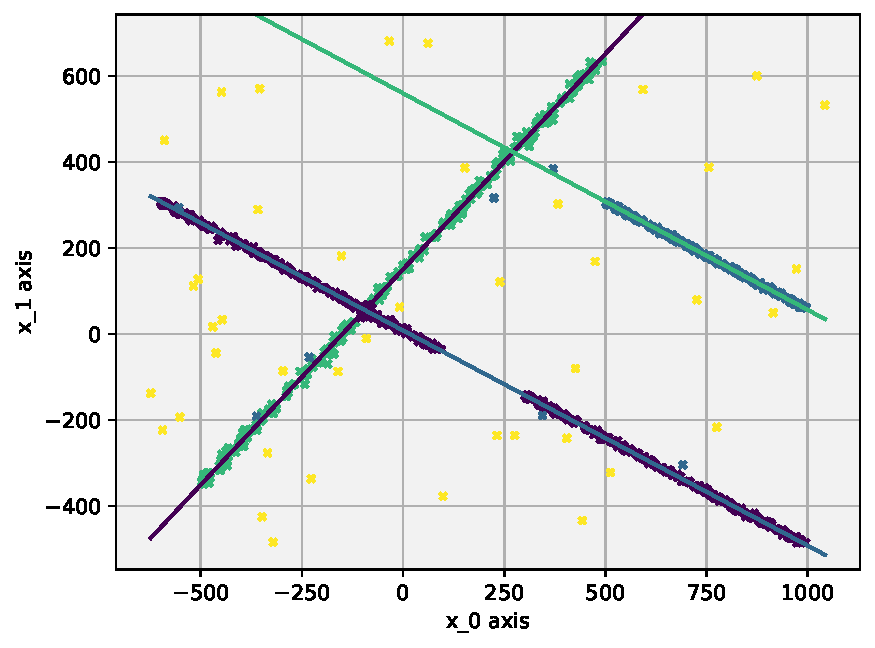
\includegraphics[width=.7\textwidth]{figure_method_grid/RelabeledCorrelationsWithColoredCorrs.pdf}
    \caption{Relabelled $DS$, which reassigns all previously pruned points close to Correlations found in \autoref{fig:stitchedcorr}. This represents the global correlation clustering.}
    \label{fig:relabelledcorr}
\end{figure}

\subsection{Summary}
To recap, our algorithm consists of four steps: density-based clustering, local evaluation of dense clusters, stitching of found correlations to create global correlation clusters and finally the reevaluation of previously pruned points. Since each of these components require their own specific set of parameters, our algorithm requires the user to specify several input parameters:
\begin{itemize}[label={\tiny\raisebox{1ex}{\textbullet}},topsep=6pt,itemsep=-1ex,partopsep=2ex,parsep=2ex]
    \item \text{Partitioning:} $MinPts$ and $\epsilon$-distance for \gls{optics} ordering and a $reachability_{\tau}$ to split the ordering after significant jumps
    \item \text{Local Correlation Clustering:} $s$ splits, $m$ minimum points and $j$ jitter for \gls{cash}
    \item \text{Stitching:} $\tau_{\Delta cos-dist}$ and $\tau_{\Delta eucl-dist}$ for similarity constraints
    \item \text{Relabelling:} $j$ jitter of local Correlation clustering (same as above)
\end{itemize}
\todor{selbe terminology?}
Given our algorithm's components, the worst case runtime complexity consists of the following:
\begin{itemize}[label={\tiny\raisebox{1ex}{\textbullet}},topsep=6pt,itemsep=-1ex,partopsep=2ex,parsep=2ex]
    \item \gls{optics}: $\mathcal{O}(|DS|^2)$
    \item \gls{cash}: $\mathcal{O}(2^d)$
    \item stitching: $\mathcal{O}(c^2)$
    \item relabelling: $\mathcal{O}(|DS| \cdot c)$
\end{itemize}

Summarized our agglomerated algorithm's complexity results in the sum of its components complexities, $\mathcal{O}(|DS|^2+2^d+c^2+|DS|\cdot c)$, where \gls{cash} marks the dominant factor.
Therefore just looking at the complexity, in theory, our algorithm should perform slower than the original, free of overhead \gls{cash}. However, due to the previous partitioning of the data space, we expect that the algorithm does not perform an additional $|DS|^2+c^2+|DS|\cdot c$ time slower than the original \gls{cash} considering the independent evaluation of each separate local \gls{cash} performs faster than the evaluation of the whole data space. This is due to the irrelevant candidates in \gls{cash}s parameter space, e.g. noise or points belonging to other correlations far way, being considered less often.

% Please add the following required packages to your document preamble:
% \usepackage{booktabs}
% \usepackage{graphicx}
\begin{table}[]
\centering
\resizebox{\textwidth}{!}{%
\begin{tabular}{@{}|l|l|l|@{}}
\toprule
Step                         & Parameters                                         & Complexity \\ \midrule
Partitioning                 & \begin{tabular}[c]{@{}l@{}}$\epsilon$ : Epsilon-distance\\ $MinPts$: min \# of pts in dense neighbourhood\end{tabular} & $\mathcal{O}(|DS|^2)$          \\ \midrule
Local Correlation Clustering & \begin{tabular}[c]{@{}l@{}}$s$: \# of splits\\ $m$: min \# of pts in ROI of parameter space\\ $j$: jitter\end{tabular}  & $\mathcal{O}(2^d)$          \\ \midrule
Stitching                    & \begin{tabular}[c]{@{}l@{}}$\tau_{\Delta cos-dist}$: orientation threshold\\ $\tau_{\Delta eucl-dist}$: distance threshold\end{tabular}  & $\mathcal{O}(c^2)$          \\ \midrule
Relabelling                   & $j$: jitter                                                  & $\mathcal{O}(|DS| \cdot c)$          \\ \bottomrule
\end{tabular}%
}
\caption{Summary of our algorithm's steps, their individual parameters and complexities}
\label{tab:componentsummary}
\end{table}